\documentclass[output=collectionpaper]{langsci/langscibook}

\author{Francesca {Di Garbo}\affiliation{Stockholm University}\lastand Matti Miestamo\affiliation{University of Helsinki}}%
\title{The evolving complexity of gender agreement systems}

\abstract{This paper proposes to integrate the diachronic dimension to the typological study of gender complexity, and focuses on the morphosyntactic encoding of gender distinctions via agreement patterns. After investigating the processes of language change that foster the reduction, loss, expansion and emergence of gender agreement in a sample of fifteen sets of closely related languages (N= 36 languages), we discuss how gender agreement systems in decline and on the rise pattern in terms of complexity. We show that declining and emerging gender agreement systems may exhibit increase or decrease in complexity and discuss how this relates to the fact that they represent transitional stages between absence of gender and full-fledged gender systems. In our analysis, we make use of typological implicational hierarchies in the domain of agreement as a tool to account for diachronic variation and for the patterns of simplification/complexification in the agreement systems of the sampled languages.
\medskip

\keywords{agreement hierarchy, agreement redistribution, gender emergence, gender expansion, gender loss, gender reduction, morphophonological erosion, complexification, simplification}
}%
\begin{document}
\maketitle


\section{Introduction and key notions}
\label{intro2}
Within the last decade, pioneering research on the complexity of grammatical gender has contributed to identify a number of dimensions along which gender systems may vary in complexity (see \citealt{Audring2014,Audring2017,DiGarbo2016} for gender-specific complexity measures\footnote{In%
  addition, see \citet{Passer2016b} for a discussion of gender complexity in comparison with other nominal classification strategies; and \citet{Leufkens2015} for a discussion of grammatical gender in the context of a general model of complexity and transparency in grammar.}%
), and to apply these dimensions of complexity variation to research on the typology of gender systems within specific language families and areas of the world \citep{DiGarbo2016}. The approach followed in these studies has been predominantly synchronic. In this paper, we argue that integrating the diachronic dimension to the typological study of gender complexity is essential to understand how gender systems vary in complexity (i.e., along which dimensions of the proposed metrics) and how this variation is distributed crosslinguistically.

We investigate the evolution of complexity in the domain of grammatical gender by using a diachronic approach to the study of linguistic diversity in line with \citet{Greenberg1978a}. Greenberg addressed possible pathways of change between different types of structures and languages and argued that there would likely be a diachronic connection between all language types in a typology in the sense that change from any given type to any other type would be possible. This diachronic route would not always be direct, but rather mediated by other types, and the relative stability of the different types would differ, with some types qualifying as \textit{stable, persistent}, and others as \textit{unstable, transitional}. In this paper, we describe the patterns of language change whereby complexification and simplification in gender systems take place, explore possible functional explanations to the unfolding of these changes, and show how these explanations are ultimately grounded in well-known implicational tendencies in the typology of gender systems. In addition, by operationalizing gender complexity as a dynamic, evolving variable, we explore the relationship between the complexity and stability of gender systems.\footnote{On the stability of gender systems see the pioneering large-scale typological investigation by \citet{Nichols1992} as well as the more recent overview by \citet{Nichols2003}. For a study of the diachrony and stability of grammatical gender in the \ili{Indo-European} family, see \citet{Matasovic2004}.} The questions we attempt to answer are:
\begin{itemize}
\item Which complexities are most stable in the domain of grammatical gender?
\item Which other aspects of gender complexity are more likely to change?
\item To what extent can we identify complexification or simplification in the processes of emergence and expansion of gender on the one hand, and reduction and loss of gender on the other?
\end{itemize}

Following \citet{Miestamo2006,Miestamo2008} we define complexity in absolute, theory-oriented, objective terms, paying attention to the number of elements in a system and connections between these.
In an information-theoretic perspective, complexity can ultimately be reduced to description length: of two entities, for instance two grammatical systems, the less complex one is the one whose shortest possible description is shorter. In other words, the simpler entity can be compressed into a smaller space without losing information. This approach also aligns with complexity theories outside linguistics and thereby allows linguistic complexity to be viewed in a cross-disciplinary perspective as well.
%In information-theoretic terms, complexity can ultimately be reduced to description length: of two entities, e.g., grammatical systems, the less complex one is the one whose shortest possible description is shorter. In other words, the simpler entity can be compressed into a smaller space without losing information. This information based view of complexity is known as Kolmogorov Complexity \citep[see][]{Li1997}. To take a very simple example, a phoneme system that has more members and whose minimal description takes more space, is more complex in this respect than one with fewer members and a shorter minimal description. Speaking about overall complexity, to put things simply for the sake of illustration, assuming we have complete, comprehensive and adequate descriptions of languages, the language with the thinnest grammar book will be the least complex in terms of grammar and the one with the thickest book, will be the most complex.
%The notions of cost and difficulty of processing and learning are related to complexity, but as \citet{Dahl2004} points out, it is important to keep these apart. Some authors, e.g., \citet{Kusters2003}, equate complexity with cost and difficulty, defining as complex those aspects of language that increase processing load and learning difficulty. This is what Miestamo (\citealt*{Miestamo2006}; \citealt*{Miestamo2008}) has called the relative (user-oriented, subjective) approach to complexity.
The notions of cost and difficulty of processing and learning are related to complexity, and some authors, such as \citet{Kusters2003}, take a relative, user-oriented, subjective approach, equating complexity with cost and difficulty. In a user-oriented approach, those aspects of language that increase processing load and learning difficulty are defined as complex. \citet{Dahl2004} and \citet{Miestamo2006,Miestamo2008} discuss some obvious problems with the cost- and difficulty-based approach and point out that it is important to keep the notions of complexity and difficulty apart.
%\textbf{There are some obvious problems with the relative approach. Firstly, what is costly or difficult, depends on whose perspective we take. A phenomenon that may increase the processing load of encoding, may ease the task of decoding a message. L2 learners may experience difficulties with different structures than L1 learners. If complexity is defined in such user-oriented fashion, one will have to choose the perspective of one particular user group, and this varies from researcher to researcher according to the research question and point of view (for Kusters, complexity equals the difficulties encountered by L2 learners). Secondly, not enough psycholinguistic work has been done to have a full enough picture of what is easy and what is difficult or costly. Cost and difficulty cannot, therefore, provide a general and neutral definition for complexity.}
%
However, to what extent and in what ways complexity and difficulty are correlated is a highly interesting question. We believe that keeping these notions apart is a prerequisite for adequately addressing this issue.

%Different ways of measuring grammatical complexity have been proposed in the literature \citep{Kusters2003,McWhorter2001,McWhorter2007}.
%\citet{McWhorter2001} proposed a metric for measuring the overall grammatical complexity of a language. The metric pays attention to the number of marked phonemes, to the number of syntactic rules, to the number of semantic/pragmatic distinctions made grammatically, and to the extent inflectional morphology is used. A more recent formulation \citep{McWhorter2007} has three criteria: Overspecification (``marking of semantic categories left to context in many or most languages, such as evidential marking''), Structural elaboration (``number of rules mediating underlying forms and surface forms,
%such as morphophonemics'') and Irregularity. McWhorter’s criteria are primarily meant for measuring the overall grammatical complexity of a language, but as suggested in \citet{Miestamo2006a}, they can be used for talking about the complexity of specific functional domains, such as tense-aspect-modality – or gender. \citet{Kusters2003} proposes three principles the violation of which means higher complexity: Transparency – clarity of the relation between meaning and form, Economy – restriction of the number of overtly signalled categories, and Isomorphy – identity of the order of elements in different domains. Although these principles were proposed in a study focusing on verbal inflection, they can be applied more generally as well. As noted above, Kusters uses these principles with a relative approach to complexity, but as \cite{Miestamo2008} points out, the principles of Transparency and Economy, and some aspects of Isomorphy, are easily translatable to an absolute approach.
\citet{Miestamo2006,Miestamo2008} proposes two principles by which grammatical complexity can be measured:

\begin{itemize}
\item The Principle of Fewer Distinctions, which, paying attention to grammatical meaning, defines as less complex a grammatical system in which, other things being equal, fewer semantic/pragmatic distinctions are made grammatically.
\item  The Principle of One-Meaning–One-Form, which, paying attention to the relationship between meaning and form, defines as less complex those systems and structures in which, other things being equal, each meaning is expressed by one form and each form corresponds to only one meaning.
\end{itemize}
Violations of these two principles increase complexity.

To take some examples, by the Principle of Fewer Distinctions, a gender system with two grammaticalized gender distinctions is less complex in this respect than a gender system with, say, five grammaticalized distinctions. By the Principle of One-Meaning–One-Form, we can identify a higher degree of complexity in a gender system system in which: (a) the formal expression of one or more genders is combined with other categories in one morpheme (fusion, multiple exponence); (b) one or more gender distinctions are expressed with multiple/discontinuous morphemes (fission); (c) the markers of one or more gender distinctions show two or more variants (allomorphy); and/or (d) the markers of some gender distinctions are identical in some grammatical contexts (syncretism).

While the Principle of One-Meaning–One-Form can handle the relation between meaning and form relatively exhaustively (relevant subcriteria need of course to be defined and refined), the Principle of Fewer Distinctions only covers parts of complexity on the level of meaning. Things get more complicated when we look at the interaction between different functional domains (e.g., gender and number). \citet{Dahl2004} discusses the notion of choice structure, i.e.\ the dependency of available choices on choices made earlier (cf.\ also the notion of dependency hierarchies by \citealt{Aikhenvald1998}). To take an example from the domain of grammatical gender, in many languages gender distinctions are available only in the singular, but are neutralized in the plural. This is, for instance, the case in \ili{Russian} (\ili{Indo-European}, \ili{Slavic}). In order to account for interactions between functional domains and their effect on the complexity of individual domains, \citet{DiGarbo2014,DiGarbo2016} proposes the Principle of Independence.
\begin{itemize}
    \item The Principle of Independence defines as less complex those systems and structures which, other things being equal, are \textit{independent} of other systems and structures.
\end{itemize}
Under the Principle of Independence, a gender system whose formal realization is dependent on number distinctions is more complex than a gender system which is not constrained by number distinctions.

The three principles, the Principle of One-Meaning–One-Form, the Principle of Fewer Distinctions, and the Principle of Independence, are all operationalized in the gender complexity metric proposed by \citet{DiGarbo2014,DiGarbo2016}, as well as in the discussion of gender complexity and canonicality by \citetvo{chapters/02}.\footnote{\citetvo{chapters/02} uses a different terminology for the Principle of One-Meaning--One-Form and the Principle of Fewer Distinctions. In her own terminology, these are the Principle of Transparency and the Principle of Economy, respectively.} In this paper, we will be especially concerned with the way in which morphosyntactic and semantic properties of reducing and emerging gender systems may be accounted for as violations of one of these principles.

The paper is organized as follows. \sectref{sec:dgm:evolution} presents some of the parameters along which gender systems may vary, and the sampling method followed in the study. In \sectref{sec:dgm:EvAgr}, attention is given to the factors that explain synchronic variation in the domain of gender agreement and to the extent to which these can be mapped on diachronic change, too. Reducing gender agreement systems are presented in \sectref{subsec:Reducing} whereas \sectref{subsec:emerging} focuses on emerging gender agreement systems, and \sectref{subsec:expanding} on expanding gender agreement systems. In  \sectref{sec:dgm:simple/compl}, we discuss how changes in the domain of gender agreement affect the complexity of gender systems. Concluding remarks are given in \sectref{sec:dgm:conclusion}.



\section{The evolution of gender complexity}
\label{sec:dgm:evolution}

In this paper, we explore synchronic distributions of types of gender systems among closely related languages, and, based on these synchronic distributions, we try to infer how gender systems change through time becoming more or less complex. We draw our observations from a sample of fifteen language sets. Each set consists of two to three genealogically related languages. In addition, the sample includes one isolate within the \ili{Austronesian} family, \ili{Chamorro}, and one mixed language, \ili{Michif}. The total number of languages is 36. The map in \figref{fig:dgm:sample} illustrates the geographic distribution and genealogical affiliations of the sampled languages. A list of the sampled languages can be found in Appendix \ref{appendix}.



\begin{figure}
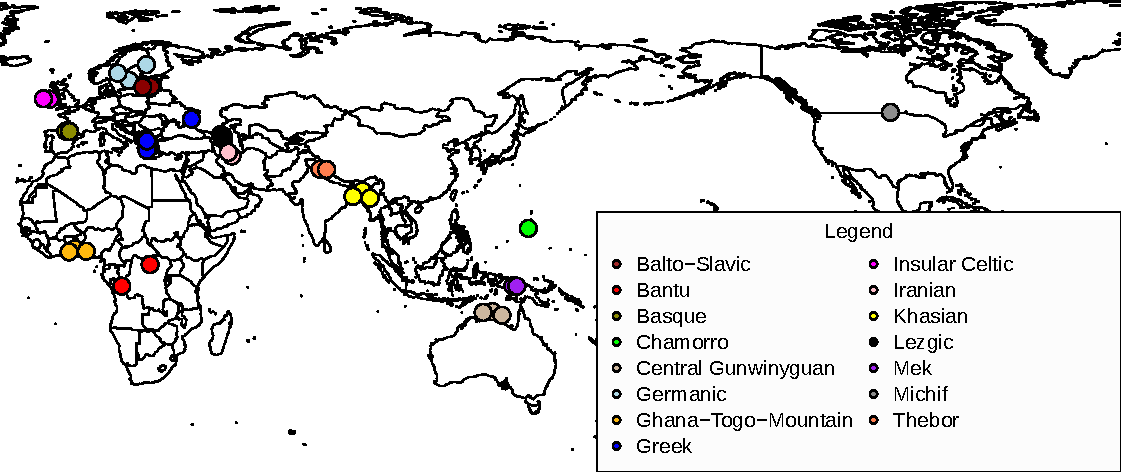
\includegraphics[width=\textwidth]{figures/11/VolumeSample1a}
\caption{The language sample}
\label{fig:dgm:sample}
\end{figure}

The data set studied stems from a larger project on the sociohistorical correlates of the evolution of gender complexity led by Francesca Di Garbo (for details, see \citealt{DiGarboinpreparation}). The diachronic processes examined in the study are somewhat biased towards instances of contact-induced change, even though language-internal developments are also discussed. While the pace and nature of these developments may thus be specific to the type of contact situation in which they unfold, we believe that the data set under study offers insights of rather general relevance with respect to the diachrony of gender marking systems. Data were collected based on a questionnaire \citep{DiGarbo2015a}, as well as on consultation of reference grammars and language experts.
%For some of the sampled language sets (especially those from Europe), diachronic inference based on observations of synchronic typological distributions is also supported by historical data.

Typological research on grammatical gender systems  has mostly focused on three broad domains of analysis:
\begin{itemize}
\item Number of genders
\item Number and/or type of gender assignment rules
\item Formal marking through agreement patterns.
\end{itemize}
We argue that these domains of synchronic variation can also be used to investigate how gender systems change through time. However, we suggest that any change in the number of gender values or the number and nature of gender assignment rules must ultimately hinge on variation and change in the domain of agreement patterns, that is, in the morphosyntactic encoding of gender distinctions. For instance, a gender value is lost when the corresponding gender agreement patterns fall out of use. Similarly, changes in the nature and distribution of gender assignment rules are reflected by the gender agreement patterns that the nouns affected by these changes trigger in discourse. For instance, we know that a former masculine noun is re-analyzed as neuter if patterns of neuter agreement are selected when the noun is used. Thus, we argue that studying synchronic and diachronic variation in patterns of gender agreement enables us to make generalizations about variation and ongoing change in the number of genders and/or the nature of the gender assignment rules that languages have. This suggestion aligns with recent observations in the literature on gender complexity where complexity in the domain of gender agreement has been shown to interact with complexity at the level of gender values and assignment rules \citep{Audring2017,DiGarbo2016}.\footnote{For instance, \citet{DiGarbo2016} shows that manipulable gender assignment tends to presuppose rather pervasive gender agreement systems in the languages of her sample.}

We explore simplification and complexification of gender systems by focusing on reducing, emerging and expanding patterns of gender agreement. The sample languages are thus selected so as to represent instances of (1) reduction, (2) loss, (3) emergence, and (4) expansion of gender agreement. These are then compared with instances of retention or lack of gender agreement as attested in closely related languages. Naturally, loss, reduction and expansion presuppose the pre-existence of a gender system within the relevant language sets, whereas emergence of gender presupposes absence of gender within the relevant language sets.  The data in \tabref{tb:patterns} and the map in \figref{fig:dgm:patterns} illustrate how the patterns of change in focus are distributed within the languages of the sample.\footnote{For language classification we follow the Glottolog \citep{Hammarstroem2018}.}


\begin{longtable}{lll}
\caption{Patterns of change attested in the languages of the sample\label{tb:patterns}}\\
\lsptoprule
Family by macroarea & Language & Pattern of change\\\midrule\endfirsthead
\midrule Family by macroarea & Language & Pattern of change\\\midrule\endhead
\endfoot\lspbottomrule\endlastfoot
Eurasia &&\\
\midrule
\ilit{Khasian}&  \ilit{Khasi}& Expansion\\
&\ilit{Lyngngam}& Retention\\
&\ilit{Pnar}&Expansion\\
% \midrule
\ilit{Basque} & Standard \ilit{Basque}&Lack\\
&Lekeitio Basque\il{Basque, Lekeitio}&Emergence\\
% \midrule
\ilit{Balto-Slavic}& \ilit{Latvian}&Retention\\
& Tamian \ilit{Latvian}&Loss\\
% \midrule
\ilit{Greek}& Modern \ilit{Greek}&Retention \\
&Pontic Greek\il{Greek, Pontic} & Reduction\\
&Rumeic Greek\il{Greek, Rumeic} &Reduction\\
&Cappadocian Greek\il{Greek, Cappadocian}& Loss \\
% \midrule
Insular \ilit{Celtic} &  \ilit{Irish}& Reduction\\
& \ilit{Irish} (Ros Much)&Retention\\
% \midrule
North \ilit{Germanic} & \ilit{Elfdalian}& Retention\\
&Karleby \ilit{Swedish} & Reduction\\
&Standard \ilit{Swedish}& Reduction\\
% \midrule
Northwestern \ilit{Iranian} &  \ilit{Eshtehardi}& Expansion\\
&\ilit{Kafteji}& Expansion \\
&\ilit{Kelasi}&Loss \\
% \midrule
\ilit{Lezgic} & \ilit{Archi}&  Retention \\
&\ilit{Aghul}& Loss\\
& \ilit{Udi}& Loss\\
% \midrule
\ilit{Thebor} &  \ilit{Shumcho}& Emergence\\
& \ilit{Jangshung}&Emergence\\
\tablevspace

Papunesia &&\\
\midrule
\ilit{Chamorro} & \ilit{Chamorro}& Emergence\\
% \midrule
\ilit{Mek} & \ilit{Nalca}&Emergence\\
&\ilit{Eipo}&Emergence\\
\tablevspace

Africa &&\\
\midrule
\ilit{Bantu} &  Kinshasa \ilit{Lingala}& Reduction\\
& Makanza \ilit{Lingala}& Expansion\\
% \midrule
\ilit{Ghana-Togo-Mountain} &  \ilit{Selee}& Retention\\
&\ilit{Igo}& Reduction (near loss)\\
& \ilit{Ikposo}& Loss\\
\tablevspace

Australia &&\\
\midrule
 Gunwinggu & \ilit{Kunwinjku} &Retention\\
&\ilit{Kundjeyhmi}& Reduction \\
&\ilit{Kune}& Loss \\
\tablevspace

North America&&\\
\midrule
Mixed Language &  \ilit{Michif}&Expansion\\ 
\end{longtable}

\begin{figure}
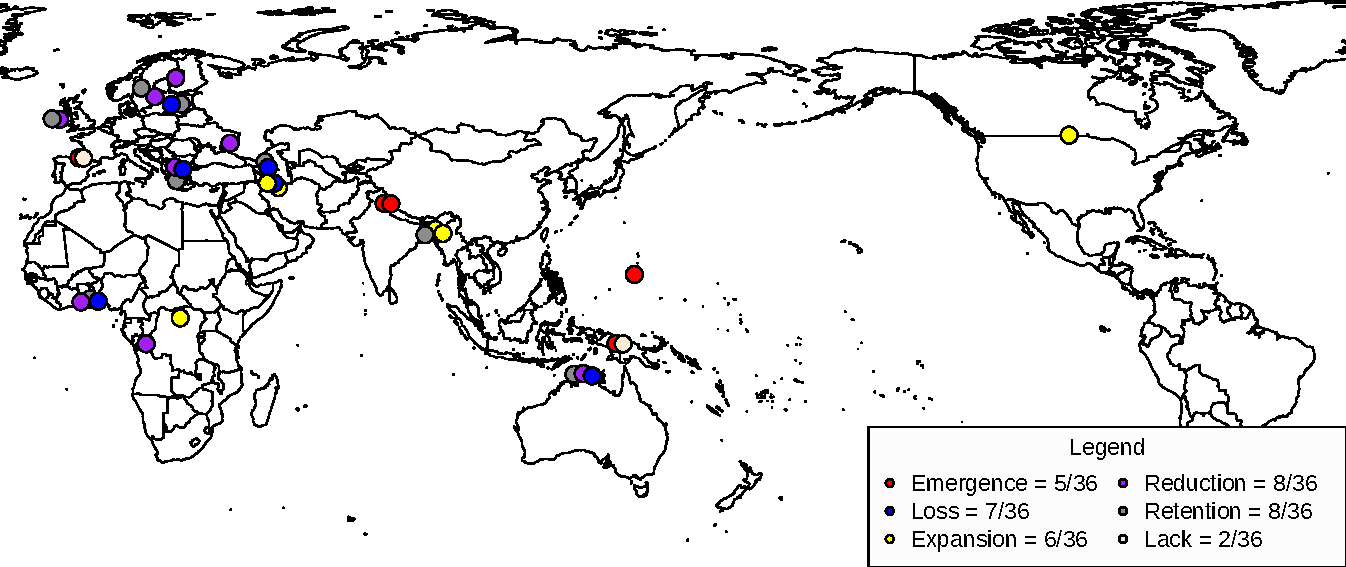
\includegraphics[width=\textwidth]{figures/11/Patterns_samplea}
\caption{Distribution of patterns of change}
\label{fig:dgm:patterns}
\end{figure}

\largerpage
It can be hypothesized that gender agreement systems in decline represent instances of reducing complexity, while gender agreement systems on the rise or under expansion represent instances of increasing complexity. A further possible hypothesis is that gender agreement systems on the rise or in decline are less complex than the more pervasive systems that they are moving towards or away from. We will come back to these hypotheses in \sectref{sec:dgm:simple/compl} and evaluate them against our data.



\section{The evolution of gender complexity in the domain of agreement}
\label{sec:dgm:EvAgr}
\largerpage
Starting with the pioneering work by \citet{Corbett1979,Corbett1991}, a great deal of research has focused on unraveling constraints on the distribution of gender distinctions on different types of agreement targets. This research has shown that certain agreement targets (e.g., personal pronouns) are more likely than others (e.g., attributive modifiers) to index semantic rather than grammatical properties of nouns.
%Aattributive modifiers exhibit higher syntactic cohesion with the controller nouns than the former type of targets (personal pronouns).
In the terminology proposed by \citet{Corbett1979,Corbett1991}, this is known as an opposition between \textit{semantic} and \textit{syntactic} agreement patterns. Preferences towards semantic or syntactic agreement per type of agreement target are captured in the form of an implicational hierarchy, which is known as the Agreement Hierarchy. The Agreement Hierarchy \textendash{} illustrated in (\ref{ex:dgm:1:AgreHie}) \textendash{} was first proposed by \citet{Corbett1979} and is further discussed in \citet{Corbett1991,Corbett2000,Corbett2006}. It expresses the likelihood of semantic agreement to occur with different types of agreement targets as well as the degree of syntactic cohesion between agreement targets and their controllers.

\ea\label{ex:dgm:1:AgreHie}
The Agreement Hierarchy (adapted from \citealt{Corbett2010})\\
\begin{itemize}

\item \spterm{Semantic Agreement}\\
attributive {\textgreater}  predicate  {\textgreater} relative pronoun {\textgreater} personal pronoun

\item \spterm{Syntactic Cohesion}\\
attributive  {\textless} predicate {\textless} relative pronoun {\textless}  personal pronoun

\end{itemize}
\z

The directions of the arrows \textendash{} ``{\textgreater}'' or ``{\textless}'' \textendash{} stand for different directionalities in the two main chains of implications entailed by the hierarchy. The first row indicates that semantic agreement on any of the targets to the left implies the presence of semantic agreement on the targets to the right, with attributive modifiers being the least likely candidate for semantic agreement. The second row  indicates that syntactic cohesion between nouns and any of the targets to the right of the hierarchy implies at least the same level of syntactic cohesion with any of the targets to the left, with personal pronouns being the agreement targets with the loosest syntactic integration to nouns.
These hierarchical effects are connected with the fact that pronouns tend to be linearly more distant from their antecedents (low syntactic cohesion) as compared, for instance, with definite articles (high syntactic cohesion), which tend to occur linearly closer to the controller nouns.\footnote{Different types of agreement targets may occur within the noun phrase (articles, quantifiers, numerals etc.\@) and further hierarchical effects between such targets cannot be excluded. This, however, falls outside the scope of the present investigation.} Pronouns are therefore more prone to index semantic properties of the discourse referent rather than lexico-grammatical properties of nouns, such as grammatical gender. Mismatches between the agreement patterns associated with different types of targets are especially likely to occur when the controller nouns are \textit{hybrid nouns}. In the case of gender, these are nouns whose inherent gender assignment is in conflict with their semantics. A classic example is the \ili{German} noun for `girl', \textit{M\"adchen}, which is grammatically neuter, but denotes a human entity. Let us consider the types of gender agreement mismatches attested in \ili{German} with the noun \textit{M\"adchen}.


\ea\label{ex:dgm:2:madchen}
\langinfo{German}{\ili{Indo-European}, Germanic}{\citealt[228]{Corbett1991}}\\
\gll Schau dir dieses Mädchen an, wie gut sie/es Tennis spielt.\\
     look you this.\textsc{n} girl at, how good she/it tennis plays\\
\glt `Look at this girl, see how well she plays tennis.'\\
\z

The example shows that while gender agreement within the noun phrase (i.e., on the demonstrative) can only conform to the lexical gender of the noun (\textit{dieses}, \textsc{n}), 
\rephrase{with the personal pronouns, speakers can choose between feminine and neuter agreement.}{speakers can choose between feminine and neuter agreement for personal pronouns. }
Feminine agreement indexes the fact that the discourse referent is female (as in \textit{sie}, \textsc{f}); neuter agreement indexes the fact that the noun for `girl' is grammatically neuter (as in \textit{es}, \textsc{n}).\footnote{\citet[228]{Corbett1991} further mentions that the older the age of the young woman that is being talked about, the more likely it is for speakers to use feminine agreement.}  Conflicts between ``semantic'' and ``syntactic'' agreement can also be understood in terms of mismatches between \textit{referential} and \textit{lexical} gender, as these terms are used by \citet{Dahl2000a} \citep[see also the study of the evolution of gender marking in medieval \ili{English} by][]{Siemund2011}.

There are at least two ways in which the Agreement Hierarchy can be used to describe synchronic variation in gender complexity, one pertaining to the types and number of attested agreement domains, and one pertaining to the type and number of preferred agreement patterns per domain. Concerning type and number of attested agreement domains, a language that exhibits gender agreement in all the agreement domains represented along the hierarchy is, in this respect, more complex than a language that, other things being equal, has agreement in fewer domains. This is, for instance, the way in which the amount of gender agreement or gender indexation is treated in the metric proposed by \citet{DiGarbo2016}.\footnote{For some observations on possible  implicational tendencies constraining which agreement domains are more likely to be targets of gender marking in a sample of 20 languages from New Guinea see \citetvo{chapters/09}.} Concerning type and number of preferred agreement patterns, a language in which gender agreement is only syntactic with all agreement targets is, in this respect, less complex than a language that, other things being equal, exhibits variation between syntactic and semantic agreement at any point along the hierarchy. For a broader discussion about the use of typological implicational hierarchies as cross-linguistic measures of complexity, see \citet{Miestamo2009}.

In this paper, we explore the extent to which not only synchronic, but also diachronic variation in the domain of gender agreement can be mapped onto the Agreement Hierarchy \citep[for an overview of the role of the Agreement Hierarchy in the diachrony of nominal classification see also][]{Seifart2010}.  With respect to types and number of agreement domains, we find that, in the languages of our sample, both the rise and the decline of gender agreement tend to start off from the agreement domains at the two opposite ends of the Agreement Hierarchy, i.e., either from attributive modifiers or from personal pronouns and/or other type of anaphoric constructions, such as light nouns with anaphoric functions (for the latter, see also \citealtv{chapters/12}). With respect to types and number of preferred agreement patterns per domain we find that, in the languages of the sample, at least the decline and loss of gender agreement tend to be directional, and that the attested lines of directionality are reminiscent of the two opposite pulling forces described by the Agreement Hierarchy: syntactic cohesion between controllers and targets, and spread of semantic agreement. However, we make no claims about the universality of these tendencies, and we do not exclude that, in languages other than those sampled for this study, diachronic change in the morphosyntax of gender agreement occurs on other types of agreement targets first. Finally, while we argue that the hierarchy is a useful tool to \textit{describe} tendencies in how gender marking systems change, we make no claims about it having a \textit{predictive/explanatory} value concerning the spreading of such changes. On the contrary, we argue that explanations should be sought in the realm of those functional pressures that are reflected in the hierarchy.


In \sectref{subsec:Reducing}, we focus on reducing gender agreement systems; emerging gender agreement systems are discussed in \sectref{subsec:emerging} whereas the expansion of gender agreement patterns is treated in \sectref{subsec:expanding}.


\section{Reducing gender agreement systems}
\label{subsec:Reducing}
\largerpage
\subsection{Attested processes of change}
In our data, the reduction and, in some cases, the loss of gender agreement result from two distinct diachronic processes: (1) \textit{morphophonological erosion} and (2) \textit{redistribution} of agreement patterns.


By morphophonological erosion we refer to the wholesale patterns of change that lead to the loss of inflection. Sound changes (e.g., changes in stress patterns resulting in the loss of word-initial or word-final segments) can cause loss of segmental morphology, which ultimately determines the neutralization of previously overtly coded grammatical distinctions and the overall restructuring of inflectional paradigms. This process is also known in the literature under the label \textit{deflection}. Within the domain of nominal morphology, morphophonological erosion often affects gender marking along with the marking of other nominal inflectional features, such as number and case, which are frequently cumulatively encoded with gender. It has been suggested (see \citealt{Priestly1983} for \ili{Indo-European}; \citealt{Audring2009} for \ili{Germanic} languages) that, when morphophonological erosion affects the encoding of gender distinctions, the word classes that are likely to lose gender marking first are the nouns themselves (in case of overt gender systems), followed by the agreement targets that are more adjacent to nouns, i.e., adnominal modifiers, such as definiteness markers, demonstratives, adjectives and numerals, with definiteness markers generally being yet more stable than, say, numerals or adjectives. Personal pronouns (both dependent and independent) are more likely to retain the encoding of gender distinctions as a means to signal semantic properties of the discourse referents. In other words, under morphophonological erosion, gender agreement is more likely to be retained on those agreement targets where it is most functional to reference tracking and reference identification, i.e.\ demonstrative and/or personal pronouns. These may then tend to inflect based on semantically transparent principles of gender assignment (animacy and/or biological gender). In \ili{English}, for instance, the encoding of gender distinctions underwent massive erosion as part of a general weakening of inflectional morphology. As a result of this deflection process, gender marking was lost on all of the agreement targets (as well as on nouns) except for the personal pronouns, which nowadays signal the biological gender of discourse referents, and for the relative pronouns which make a distinction of the human/non-human type \citep{Curzan2003}.

\largerpage[-2]
By \textit{redistribution of agreement}, we refer to the process whereby one of the several agreement patterns available in a language (for instance, the neuter) starts being used with nouns that would normally trigger agreement in other genders (for instances, with nouns that are semantically inanimate, but grammatically masculine or feminine). If the redistribution of one agreement pattern comes to affect all agreement domains, and to effectively replace all the other competing agreement patterns independently of semantic or morphological properties of the controller nouns, then gender distinctions become neutralized. In many of the cases attested in our sample, the redistribution of agreement patterns appears to be at least initially semantically motivated: semantic oppositions generally pertaining to the domain of animacy start affecting the criteria according to which certain nouns trigger gender agreement on at least some targets. In general, the higher the number of nouns involved in the restructuring of the assignment criteria, the higher the chance that the overall gender assignment rules of a language may change. Similarly, the higher the number of agreement targets that align with the new assignment criteria, the more reasons to speak of an increase or decrease in the number of gender distinctions. 
For instance, when the semantic agreement patterns that are being redistributed are based on animacy, their generalization to all agreement targets may eventually lead to a bipartite, animate vs.\ inanimate, type of gender system, where gender assignment is semantically predictable. This is for instance the case of the \ili{Bantu} language \ili{Kinshasa Lingala}, in which all productive agreement targets index the animacy of the noun, whereas the nouns themselves retain prefixal remnants of the old, no longer productive system of gender distinctions (\citealt[130--132]{Maho1999}; \citealt[28--29]{Meeuwis2013}).  
In other cases, the most frequent (default) pattern of gender agreement is the one that takes over. This is for instance the case of Tamian \ili{Latvian} (\ili{Indo-European}, \ili{Balto-Slavic}), where the masculine agreement pattern has replaced nearly all instances of feminine agreement leading to loss of grammatical gender. The redistribution of agreement patterns is ultimately a process of analogical levelling: the gender agreement system of a language is restructured on the basis of the more semantically motivated and/or more frequent agreement pattern, which gradually spreads at the expenses of others.




 \begin{table}[t]
\caption{Morphophonological erosion and redistribution of agreement in the languages of the sample where gender agreement reduction and loss are attested}
\label{tab:2:defl}
\small
 \begin{tabularx}{\textwidth}{Xlll} % add l for every additional column or remove as necessary
  \lsptoprule
   & Languages & Directionality & Semantics \\ %table header  Resulting change &
  \midrule
Morphophonological erosion & Standard \ili{Swedish} & YES & NO\\ 
& \ili{Kelasi} & Not clear & NO \\ %& Gender reduction &
 \midrule
Redistribution & Cappadocian Greek\il{Greek, Cappadocian}   & YES & YES\\ %& Gender loss
 & Pontic Greek\il{Greek, Pontic}   & YES & YES\\ % &  Sem. Agr.
 & Rumeic Greek\il{Greek, Rumeic} & YES  & YES\\ % Sem. Agr.  &
& \ili{Irish} & YES  & YES\\ %& Gender reduction
 & \ili{Kune} & Not clear & \ili{No} data\\ %& Gender loss
\midrule
Both & \ili{Igo}  & YES & Not clear\\ %& Near loss
& Karleby Swedish\il{Swedish, Karleby} & Not clear & Partially \\
& \ili{Kinshasa Lingala}  & YES & YES\\ %& Gender reduction
& Tamian \ili{Latvian}  & Partially & Partially\\ %& Gender loss
\midrule
Not clear & \ili{Aghul} & -- & -- \\
& \ili{Kundjeyhmi}  & --  &--\\ %& Gender reduction
& \ili{Lezgian} & -- & -- \\
& \ili{Udi} &  -- & --\\ %Gender loss &
  \lspbottomrule
 \end{tabularx}
 \end{table}

  
\tabref{tab:2:defl} illustrates the distribution of patterns of reduction and loss of gender agreement within the languages of the sample, and specifies whether these are due to morphophonological erosion, redistribution of agreement, a combination of both, or whether the exact pattern of change cannot be inferred based on the data at our disposal. For each of the relevant languages, the table also specifies if directionality applies, and if the distribution of a given pattern of change is at any rate semantically motivated. Given the limited size of our sample, the analysis proposed here is merely qualitative and we draw no generalization based on the relative frequencies of the observed patterns of change. Examples for each of the possible scenarios are discussed in \sectref{subsubsec:deflection}, \ref{subsubsec:semanticization} and \ref{subsec:combined}.


\newpage 
\subsection{Reduction and loss by morphophonological erosion}
\label{subsubsec:deflection}
 
In Standard \ili{Swedish}, the opposition between masculine and feminine gender is retained in the inflectional paradigm of the independent third person pronouns (see \tabref{tab:3:Swedish}), but has been lost elsewhere.\footnote{In written language, a masculine suffix \textit{-e} may still sometimes be used on adjectives to mark masculine agreement.}

 \begin{table}[t]
\caption{Personal Pronouns in Standard Swedish}
\label{tab:3:Swedish}
 \begin{tabularx}{\textwidth}{XXXl} % add l for every additional column or remove as necessary
  \lsptoprule
&  M    & F & PL \\ %table header
  \midrule
Nominative & \textit{han} `he' & \textit{hon} `she' & \textit{de} `they'\\
Genitive & \textit{hans} `his' &  \textit{hennes} `her' & \textit{deras} `their'\\
Accusative &\textit{honom} `him'  & \textit{henne} `her' & \textit{dem} `them'\\
  \lspbottomrule
 \end{tabularx}
\end{table}

\largerpage[1.5]
 The Masculine and Feminine singular forms of the third person pronouns are used to signal the biological gender of human and other animate referents.\footnote{During the last decade, a biological gender-neutral form, \textit{hen} has been introduced. Its frequency of use has rapidly increased, both in written and spoken \ili{Swedish} discourse.}
With non-animate entities, the demonstrative pronouns \textit{den}, Common Gender, and \textit{det}, Neuter Gender, are used instead, and the choice between the two is based on the lexical gender of nouns. In sum, in the pronominal domain, Standard \ili{Swedish} has a four-way gender distinction: Masculine, Feminine, Common, Neuter, with a split between animate and inanimate referents governing the distribution of these gender values.  Within the domain of adnominal modification, \ili{Swedish} distinguishes between a Common and a Neuter Gender only: \textit{en person} `a person' (Common Gender), and \textit{ett hus} `a house' (Neuter Gender). Historically, the Common Gender is the result of a merger between the Feminine and Masculine genders. Many nonstandard varieties of \ili{Swedish}, as well as many other \ili{Scandinavian} varieties, retain a tripartite gender system. Tripartite gender systems were found all over Scandinavia before the standard varieties with a bipartite gender system, such as \ili{Danish} and \ili{Swedish}, started spreading.\footnote{Before the spread of the standard languages, bipartite gender systems were only attested in Denmark, southern Sweden, the M\"alaren valley in Sweden, and pockets of Norway where varieties heavily influenced by \ili{Danish} were spoken (\"Osten Dahl, personal communication).} One of the \ili{Swedish} dialects which still retains a fully productive tripartite gender system is \ili{Elfdalian}, spoken in the \ili{Swedish} region of Northern Dalarna by approximately two thousand people.\footnote{Data from \citet{AAkerberg2012}, as well as from Östen Dahl (personal communication).} In \ili{Elfdalian}, the opposition between Masculine, Feminine and Neuter gender runs productively through the whole agreement system.
A tripartite gender system of the type retained by \ili{Elfdalian} is also attested in Old \ili{Swedish} texts.\footnote{The use of the Masculine and Feminine pronouns with inanimate antecedents continued in the written language until the nineteenth century, even though this distinction was lost in all other domains of nominal inflection and no longer maintained in spoken use (\"{O}sten Dahl, personal communication).} The Masculine-Feminine merger in the domain of adnominal modification appears to be due to a combination of various morphophonological processes, such as the erosion and loss of the masculine \textit{-er} ending in the inflectional paradigm of strong adjectives, the loss of the masculine suffix \textit{-r} before the definite suffix in the nominative form of the noun, and the loss of final consonant length in the inflectional paradigm of the definite suffixes \citep[652--654]{Duke2010}. Finally, pervasive reduction in gender agreement domains is attested in Karleby Swedish,\il{Swedish, Karleby} the variety of \ili{Swedish} spoken in the town of Karleby, located in the \ili{Finnish} region of Ostrobothnia.\footnote{It is worth mentioning that, contrary to Karleby Swedish,\il{Swedish, Karleby} some other Ostrobothnian varieties of Swedish\il{Swedish, Ostrobothnian} display quite conservative gender systems (for more details see \citealt[40--50]{Hulden1972}.) However, it is perhaps unsurprising, that the near loss of gender distinctions is attested in the northernmost corner of the \ili{Swedish} speaking area of Finland.} 
\largerpage
Gender agreement reduction in Karleby Swedish\il{Swedish, Karleby} is best described as an instance of both morphophonological erosion and agreement redistribution. It is therefore discussed in \sectref{subsec:combined}.

Loss of gender in \ili{Kelasi}, a Northwestern \ili{Iranian} language of the \ili{Tatic} sub-branch, is also the result of a process of morphophonological erosion. \citet{Stilotoappear} proposes a historical-comparative analysis of gender loss in \ili{Kelasi} whereby the decline of gender marking is explained as originating from the domain of noun inflection. In \ili{Kafteji}, a closely related language spoken at a distance of twelve kilometers from \ili{Kelasi}, gender distinctions are still retained. However, in \ili{Kafteji}, overt marking of gender on nouns is dropped when nouns are used in a generic sense or as citation forms, and gender is never marked on agreement targets when these occur in isolation. Based on this comparative evidence, \citet[27]{Stilotoappear} hypothesizes that, at some point in the history of \ili{Kelasi}, gender marking became increasingly optional and ``went through gradual stages of erosion by becoming more and more rarely used in speech'', to be finally dropped in all domains of encoding. Even though the individual stages of this process of erosion are not known, nouns \textendash{} ``the crucial locus of gender in the grammar'' of \ili{Kelasi} \citep[27]{Stilotoappear} \textendash{} are viewed as the word class from which the decline of gender marking originated. This is why we classify \ili{Kelasi} as an instance of gender loss by morphophonological erosion.

The reduction and loss of gender inflections as a result of a more general erosion of nominal morphology are widely attested across different genera of the \ili{Indo-European} language family. See \citet[chapter 9]{Audring2009} for an overview of patterns of gender reduction and loss across \ili{Germanic} languages; \citet{Priestly1983} for a broader overview of the \ili{Indo-European} language family, and, in particular, of pronominal relics of the neuter gender in \ili{Romance} (e.g., \ili{Italian}, \ili{French}) and \ili{Baltic} (e.g., \ili{Lithuanian}) languages.

\subsection{Reduction and loss by redistribution of agreement}
\label{subsubsec:semanticization}
Gender reduction and loss as a result of the redistribution of agreement patterns are widely attested in our sample. In this section, we discuss a selection of the attested cases.



The Asia Minor \ili{Greek} dialects are a group of \ili{Greek} varieties that are or, prior to the 1923 population exchange between Greece and Turkey, used to be spoken in Turkey. \citet{Karatsareas2014} identifies five main dialects within the Asia Minor \ili{Greek} cluster:  Cappadocian, Pharasiot, Pontic, Silliot, and Rumeic. While the first four varieties were spoken in different areas of modern Turkey, Rumeic is the variety spoken by the \ili{Greek} inhabitants of Mariupol, Ukraine, and can be considered as the historical descendant of the Pontic spoken by \ili{Greek} settlers in Crimea.

\newpage 
Due to their long-lasting history of isolation from mainland varieties of \ili{Greek}, and, partially, to a history of prolonged contact and bilingualism with \ili{Turkish}, the Asia Minor \ili{Greek} dialects exhibit a wealth of grammatical innovations among which a significant reorganization of the gender agreement and gender assignment patterns. This is attested in all Asia Minor \ili{Greek} varieties but Silliot,\il{Greek, Silliot} which rather retains a conservative system similar to the one attested in Standard \ili{Greek} and in other Modern \ili{Greek} varieties outside the Asia Minor area \citep[83]{Karatsareas2014}. Examples (\ref{ex:dgm:3:Pontic}), (\ref{ex:dgm:4:Rumeic}), (\ref{ex:dgm:5:Pharasiot}), and (\ref{ex:dgm:6:Cappadocian}) illustrate the innovations attested in the domain of gender agreement and gender assignment in four out of the five groups of Asia Minor \ili{Greek} dialects. We present data from the dialects that display renewed gender systems and compare them with equivalent structures in Standard \ili{Greek}, where these innovations are not attested.\footnote{Notice that the Standard \ili{Greek} examples reported by \citet{Karatsareas2014} can be either full or partial translations of the corresponding example in one of the Asian Minor \ili{Greek} dialects.}

In Pontic,\il{Greek, Pontic} example (\ref{ex:dgm:3:Pontic}), the inanimate feminine noun for `door' triggers neuter agreement with agreement targets non-immediately adjacent to nouns. In the corresponding Standard \ili{Greek} sentence, agreement is feminine with all targets.

\ea\label{ex:dgm:3:Pontic}
\ea
\langinfo{Argyro\'upolis Pontic}{\ili{Indo-European}, Greek}{\citealt[79]{Karatsareas2014}}\\
\gll i p\'orta (...) m\'ono \'imoson \'oran est\'eknen anixt\'on \\
\textsc{def.f.sg} door.\textsc{f.sg} (...) only half.\textsc{n.sg} hour.\textsc{f.sg} stay.\textsc{pst.3sg} open\textsc{.n.sg} \\
\glt `The door would stay open for only half an hour.'
\ex
\langinfo{Standard Greek}{\ili{Indo-European}, Greek}{\citealt[80]{Karatsareas2014}}\\
\gll i p\'orta m\'ono mis\'i \'ora \'emene anixt\'i \\
\textsc{def.f.sg} door.\textsc{f.sg} only half\textsc{.f.sg} hour\textsc{.f} stay.\textsc{pst.3sg} open.\textsc{f.sg}\\
\glt `The door stayed open for only half an hour.'
\z
\z
In Pontic,\il{Greek, Pontic} the criteria of gender assignment are reorganized based on the animacy of the noun: semantically inanimate, but grammatically masculine and feminine nouns are to a large extent treated as neuter. This semantic reorganization is reflected at the level of agreement: semantic (neuter) agreement with inanimate masculine and feminine nouns is attested on all agreement targets but prenominal definite articles, which instead agree with the grammatical gender of the nouns (i.e.\ they take masculine or feminine inflection).

\largerpage
In Rumeic,\il{Greek, Rumeic} example (\ref{ex:dgm:4:Rumeic}), the pattern of semantic agreement observed in Pontic\il{Greek, Pontic} is generalized to all targets: the inanimate noun for `winter' (which is masculine in Standard \ili{Greek}) triggers neuter agreement with all agreement targets.

\ea\label{ex:dgm:4:Rumeic}
\ea
Rumeic (\ili{Indo-European}, Greek; \citealt[79]{Karatsareas2014})\\
\gll tu ko mas to ʃum\'os en xl\'isku\\
\textsc{def.n.sg} \textsc{poss.n.sg} \textsc{1pl.gen} \textsc{def.n.sg} winter.\textsc{n.sg} be.\textsc{prs.3sg} tepid.\textsc{n.sg}\\
\glt `Our winter is tepid.'
\ex
\langinfo{Standard Greek}{\ili{Indo-European}, Greek}{\citealt[80]{Karatsareas2014}}\\
\gll o ðik\'os mas o \c{c}im\'onas \\
\textsc{def.m.sg} \textsc{poss.m.sg} \textsc{1pl.gen} \textsc{def.m.sg} winter.\textsc{m.sg} \\
\glt `our winter'
\z
\z
In Rumeic,\il{Greek, Rumeic} the gender system has been restructured based on semantic grounds: male entities are assigned to the Masculine Gender, female entities to the Feminine and inanimate entities to the Neuter.

A different path is taken by Pharasiot\il{Greek, Pharasiot} and Cappadocian,\il{Greek, Cappadocian} where the redistribution of the neuter gender agreement pattern leads to a more pervasive erosion of the gender system. In Pharasiot,  as illustrated in example (\ref{ex:dgm:5:Pharasiot}), the animate noun for `woman' (feminine in Standard \ili{Greek}) triggers neuter agreement with all targets but the definite article adjacent to the noun.

\ea\label{ex:dgm:5:Pharasiot}
\ea
\langinfo{Pharasiot}{\ili{Indo-European}, Greek}{\citealt[79]{Karatsareas2014}}\\
\gll f\'erinke adʒ\'ino i n\'eka xort\'are \\
bring.\textsc{pst.3.sg} \textsc{dem.dist.n.sg} \textsc{def.f.sg} woman.\textsc{f.sg} herb.\textsc{pl} \\
\glt `that woman used to bring herbs.'\\
\ex
\langinfo{Standard Greek}{\ili{Indo-European}, Greek}{\citealt[80]{Karatsareas2014}}\\
 \gll ec\'ini i ʝin\'eka \\
 \textsc{dem.dist.f.sg} \textsc{def.f.sg} woman.\textsc{f.sg} \\
 \glt `that woman'
\z
\z
In Pharasiot,\il{Greek, Pharasiot} the neuter agreement has been generalized to all nominal types (animate and inanimate) and the semantic opposition between animate and inanimate entities has been neutralized. Only the agreement targets that are most adjacent to nouns retain agreement with the original grammatical gender of the noun (in this case with the Feminine).

Finally, in Cappadocian,\il{Greek, Cappadocian} example (\ref{ex:dgm:6:Cappadocian}), the neuter agreement pattern is generalized to all nouns, irrespective of animacy and type of target (the noun for `wall' is masculine in Standard \ili{Greek}).

\ea\label{ex:dgm:6:Cappadocian}
\ea
\langinfo {Ax\'o Cappadocian}{\ili{Indo-European}, Greek}{\citealt[79]{Karatsareas2014}}\\
\gll t spit\c{c}\'u ta ndix(u)s xtizm\'ena \\
\textsc{def.sg.gen} house.\textsc{sg.gen} \textsc{def.pl} wall.\textsc{pl} built.\textsc{pl} \\
\glt `The walls of the house (are) built.'\\
\ex
\langinfo{Standard Greek}{\ili{Indo-European}, Greek}{\citealt[80]{Karatsareas2014}}\\
\gll i t\'i\c{c}i ine xtixm\'eni \\
\textsc{def.m.pl} wall\textsc{.m.pl} be.\textsc{prs.3pl} built.\textsc{m.pl} \\
\glt `the walls are built'.
\z
\z

 
In Cappadocian,\il{Greek, Cappadocian} pervasive redistribution of the neuter agreement pattern has led to complete gender loss, whereby agreement patterns only index number distinctions, in this case that the noun is plural.\footnote{Feminine and masculine agreement survive in the singular form of definite articles preceding nouns only in the Delmes\'o, Pot\'amia, and S\'ilata varieties of Cappadocian \citep[97]{Karatsareas2014}.}

Using internal reconstruction, historical data, and data from contemporary varieties of Pontic\il{Greek, Pontic} spoken in Greece, \citet{Karatsareas2014} shows that two main orders of facts account for the rise and spread of semantic agreement in Pontic.\il{Greek, Pontic} On the one hand, the triggers of semantic agreement are nouns at the bottom of the Individuation Hierarchy \citep{Sasse1993}, that is, inanimate mass and abstract nouns that are grammatically assigned to the masculine or feminine genders. These are typical instances of hybrid nouns, i.e., nouns whose denotational semantics is in conflict with their grammatical gender assignment (these nouns denote inanimate entities, but are grammatically masculine or feminine).  On the other hand, according to Karatsareas' reconstruction, the spreading of semantic agreement starts from the personal (and demonstrative) pronouns. In Pontic,\il{Greek, Pontic} the sole agreement targets that are left untouched by these redistribution patterns are those that are most adjacent to nouns, i.e., prenominal definite articles. Rumeic\il{Greek, Rumeic} is the only Asia Minor \ili{Greek} dialect where semantic agreement has become generalized to all nouns and targets leading to a gender system which is still tripartite (Masculine, Feminine, Neuter), but in which assignment rules and agreement patterns are entirely semantic. Conversely, in Pharasiot\il{Greek, Pharasiot} and Cappadocian, the generalization of the neuter agreement pattern to human nouns has paved the way for a more pervasive erosion of gender marking.\footnote{A similar development is attested in some more recent varieties of Pontic,\il{Greek, Pontic} where at least human nouns denoting female referents systematically trigger neuter agreement \citep[96--97]{Karatsareas2014}. } This process of erosion has turned into complete loss in (varieties of) Cappadocian only. The loss of gender in Cappadocian \ili{Greek} is seen by \citet[99]{Karatsareas2014} as reasonably connected with the fact that, among all Asia Minor \ili{Greek} varieties, this is the one with the longest and tightest history of contact and bilingualism with \ili{Turkish}. A summary of the patterns of agreement redistribution attested in Pontic,\il{Greek, Pontic} Rumeic,\il{Greek, Rumeic} and Cappadocian\il{Greek, Cappadocian} \ili{Greek} is given in \figref{fig:dgm:AMG}.

\begin{figure}
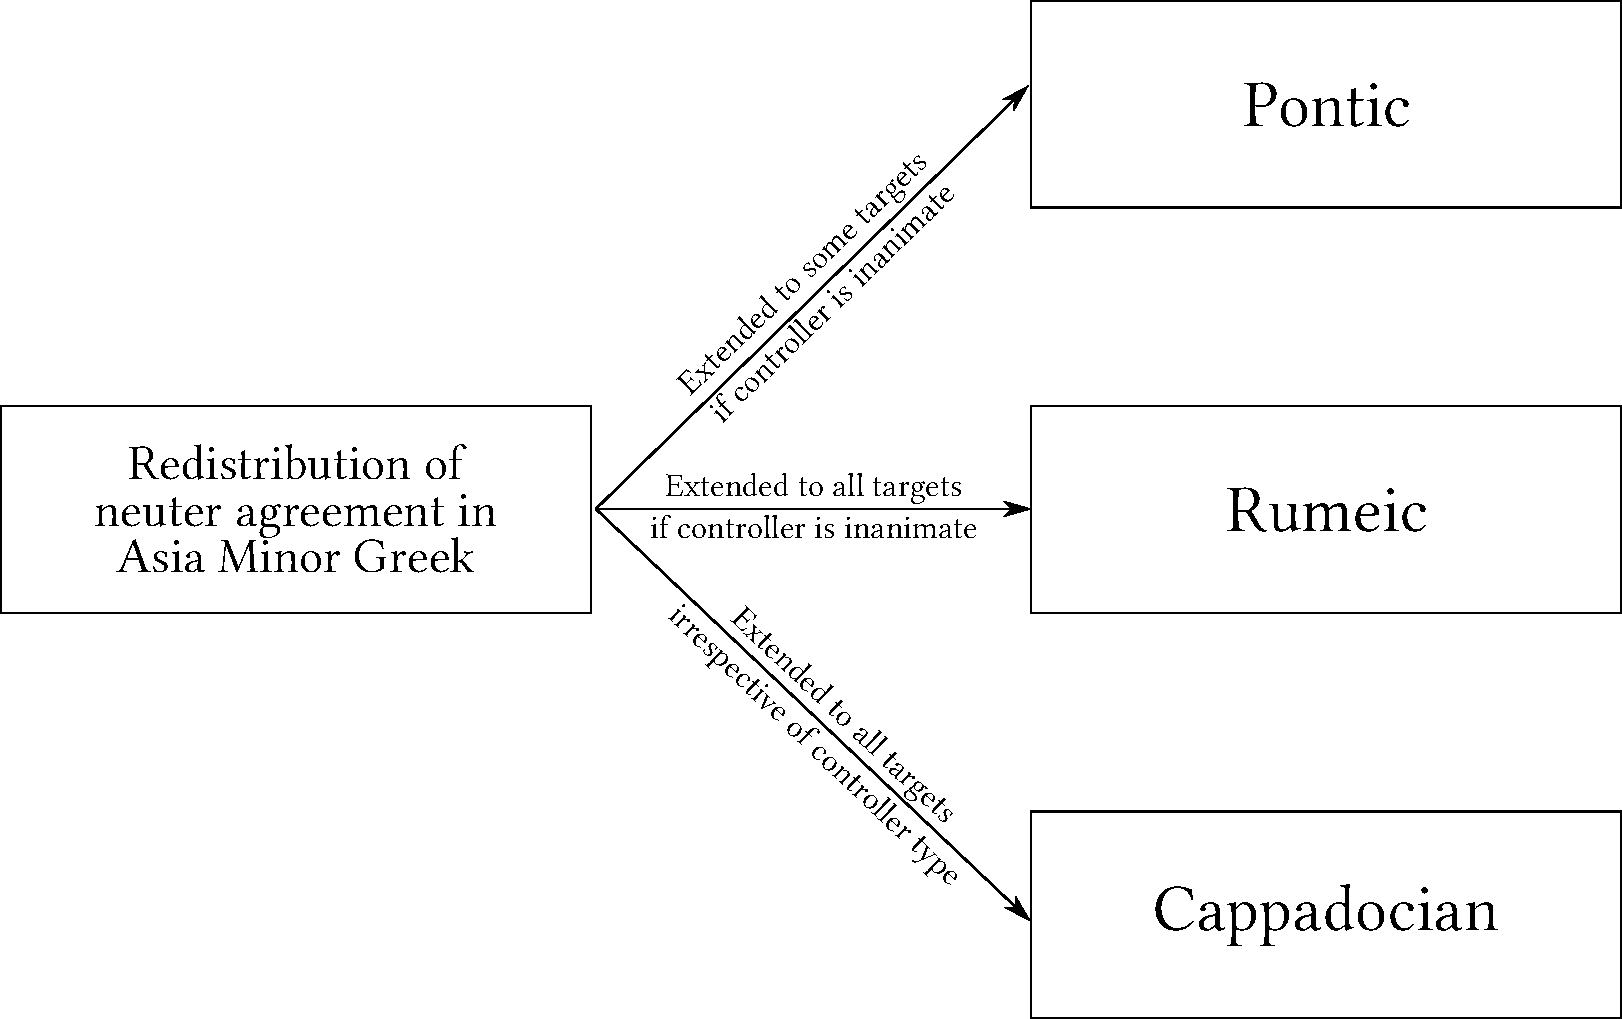
\includegraphics[height=.4\textheight]{figures/11/AMGa}
\caption{Neuter Agreement in the Asia Minor Greek dialects}
\label{fig:dgm:AMG}
\end{figure}

Semantically motivated redistribution of gender agreement patterns also occurs in contemporary varieties of urban \ili{Irish} as documented by \citet{Frenda2011}. In these non-standard varieties of \ili{Irish} (which Frenda classifies as ``non-native''), masculine agreement is increasingly used as the default agreement pattern for grammatically feminine nouns denoting inanimate entities. The redistribution is very pervasive in the domain of personal pronouns where the gender assignment system appears to be largely based on an opposition between ``female referent'' (marked by the Feminine Pronoun) and ``everything else'' (marked by the Masculine Pronoun). In the domain of adnominal modification,  controller nouns that are grammatically feminine but semantically inanimate still trigger feminine agreement (this is attested in 88\% of the examined cases; see \citealt[17, Figure 1]{Frenda2011}).

In sum, the data from our sample suggest that patterns of agreement redistribution tend to be constrained by the syntactic cohesion between controller nouns and agreement targets. Those agreement targets that are most adjacent to nouns are the ones that are affected last by the spreading of innovations.

\subsection{Combined and unclear cases}
\label{subsec:combined}
In some cases, both morphophonological erosion and agreement redistribution are attested in one and the same language, albeit not necessarily as the result of co-occurrent patterns of change.
%The last two instances of gender reduction due to semanticization of agreement in our sample, \ili{Igo} and \ili{Lingala}, bring us to Africa. For reasons of space, only the \ili{Igo} case will be discussed in detail. For an overview of the diachrony of the gender system of \ili{Lingala}, see \citet{DiGarbo2016}.  in the village of \ili{Bogo}, which is located in western Ghana at the border with Togo
One such case is \ili{Igo}, a \ili{Ghana-Togo-Mountain} language of the \ili{Kwa} subfamily of the \ili{Atlantic-Congo} family, spoken by approximately 6.000 people \citep{Gblem-Poidi2007}. In general, the \ili{Ghana-Togo-Mountain} languages represent an ideal test case for an intragenealogical study of the diachrony of gender systems and their evolving complexity (for a historical\hyp{}comparative overview, see also the contribution by \citealtvo{chapters/05}). Some languages within the family, such as \ili{Selee} \citep{Agbetsoamedo2014} and Siwi \citep{Dingemanse2009}, display very productive gender systems characterized by a high number of (non-sex-based) gender distinctions, pervasive agreement and overt marking of gender on nouns. Some other languages (e.g., \ili{Animere}) present heavily eroded and completely semanticized systems of gender assignment and gender agreement, whereby gender assignment and agreement are animacy-based, and traditional noun class marking on nouns is retained merely as a means of marking singular/plural distinctions. Finally, a few other languages, such as \ili{Ikposo} \citep{Soubrier2013}, have lost gender completely and retain relics of the extinct gender marking system only on nouns. \ili{Igo} provides us with an example of a system in transition from animacy-based gender distinctions (of the \ili{Animere} type) to complete loss of gender (of the \ili{Ikposo} type).  \citet{Gblem-Poidi2007} argues that the original gender system of \ili{Igo} consisted of eleven non-sex-based genders whose distribution paralleled the eleven pairings of singular and plural nominal prefixes still in use in the language. Nowadays, however, in formal registers of \ili{Igo},\footnote{Those in use in the literacy program and in the New Testament Translation (Honorine Gblem-Poidi, personal communication).} only an animate/inanimate type of distinction is marked on the agreement targets.
% (subject pronouns, interrogative pronouns, demonstratives, definite and indefinite markers, adjectives) except the numerals, which rather index whether the noun is human or non-human.
It can thus be assumed that this animacy-based gender system is already an eroded system, and that this process of erosion may have occurred through the spreading of semantic, animacy-based agreement. Albeit preferred in formal registers and still in use among the older generations, the animacy-based gender system of \ili{Igo} is described by \citet{Gblem-Poidi2007} as under threat, highly eroded in the speech of middle-aged speakers, and practically unused by the younger speakers. The ongoing loss of gender distinctions in \ili{Igo} is the result of the erosion of segmental gender morphology. Gender agreement morphemes are omitted in actual discourse while their tonal patterns are retained in the form of floating tones that encroach upon the immediately following tonal segments. Interestingly, in spoken use, the former animate gender agreement markers (\textit{\`u-} and \textit{b\`u-}) are resumed and reanalyzed as nominal number markers, whereby \textit{\`u-} marks the singular with both animate and inanimate nouns, and \textit{b\`u-} the plural, but only with animate nouns. Example (\ref{ex:dgm:7:Igo}) shows overt plural marking with animate nouns and zero marking with inanimate.
 
\ea\label{ex:dgm:7:Igo}
\langinfo {Igo}{\ili{Niger-Congo}, \ili{Kwa}, Ghana-Togo-Mountain}{\citealt[59]{Gblem-Poidi2007}}
\ea
%\\
\gll b\'eg\`u l\={ɔ} b\`u ɖ\={a} w\={u}l\={u}\\
children \textsc{def} \textsc{pl} \textsc{prog.sbj} dry.out\\
\glt `The children are losing weight.'\\
 
\ex
%\langinfo{Igbo}{\ili{Niger-Congo}, \ili{Kwa}, Ghana-Togo-Mountain}{\citealt[59]{Gblem-Poidi2007}}\\
\gll \={a}t\={i} l\={ɔ} ɖ\`a\={a} w\={u}l\={u}\\
trees \textsc{def} \textsc{prog.sbj} dry.out \\
\glt `The trees are dying out.'
\z
\z

Based on the data at our disposal, it is not possible to determine whether the loss of segmental gender marking affects all agreement targets at once or is gradually spreading from one agreement domain to the other.

Another instance of pervasive reduction of gender agreement morphology which seemingly results from a combination of morphophonological erosion and agreement redistribution is Karleby Swedish.\il{Swedish, Karleby} In this variety of \ili{Swedish}, gender distinctions have been lost on all agreement targets except for the definite articles (immediately adjacent to nouns) and the demonstrative and personal pronouns. These retain a tripartite distinction between Masculine, Feminine and Neuter gender. The masculine and feminine forms are however used only when the controller noun denotes human beings; in all other cases only one form (the Neuter) is used both in the domain of definite and indefinite articles and with demonstrative and anaphoric pronouns \citep{Hulden1972,Hultman1894}. It is reasonable to think that this superimposed animacy-based distinction (whereby only nouns denoting humans trigger a masculine/feminine distinction) might have spread from the domain of anaphoric pronouns (where, for instance, it is also found in Standard \ili{Swedish}) to the definite articles.



In the Tamian dialects of \ili{Latvian}, loss of gender marking is also the result of a complex interplay between morphophonological erosion and agreement redistribution. According to the recent comparative study by \citet{Waelchli2017}, the loss of short vowels in final syllables caused the neutralization of the opposition between masculine and feminine gender in the accusative plural of
nominal paradigms. The neutralization pattern later extended to the demonstratives. This paved the way to several processes of redistribution that led to the gradual generalization of masculine agreement to other types of targets (for instance, past participles and predicative adjectives), but never to all instances of gender agreement. As underscored by \citet{Waelchli2017}, and contrary to what suggested in previous literature \citep{Rudzite1980}, the unfolding of these developments varies substantially across different Tamian varieties and cannot be subsumed under one unitary model of change.



For three of the sampled languages, 
\ili{Kundjeyhmi} (Central \ili{Gunwinyguan}), 
\ili{Udi} (\ili{Lezgic}),
and 
\ili{Aghul} (\ili{Lezgic}),
the patterns of change behind the reduction and loss of gender agreement patterns cannot be fully inferred based on the data at our disposal.



\subsection{Reducing gender agreement systems: summary}


In our data, the reduction and loss of gender agreement can be described as the result of two distinct processes: morphophonological erosion and redistribution of agreement. We also found evidence for some directional effects in the way in which these developments spread. The morphophonological erosion of gender inflections tends to spread from nouns to those agreement targets that are syntactically more adjacent to nouns (i.e., adnominal modifiers). Conversely, the redistribution of agreement patterns affects anaphoric pronouns (i.e., the agreement targets that are least adjacent to nouns) first.  In our sample, these directional effects are attested across different language families and different types of gender systems, which makes it reasonable to hypothesize that they may respond to more general, possibly universal, tendencies in language change. Furthermore, we believe that these directional effects are due to two distinct types of functional constraints: the syntactic cohesion between agreement targets and their controllers, on the one hand, and the sensitivity of agreement targets to semantic properties of discourse referents, on the other hand.  The higher the syntactic cohesion (e.g.\ with definite and indefinite articles), the lower the sensitivity to referential properties, and vice versa (personal pronouns have looser syntactic cohesion with nouns and are therefore more sensitive to semantics). We suggest that the Agreement Hierarchy, a generalization over observed tendencies in the distribution of syntactic and semantic agreement, makes it possible to detect and describe the connection between these two opposite tendencies. This is because, as also outlined in \sectref{sec:dgm:EvAgr}, the two ends of the scale, attributive modifiers and personal pronouns, represent instances of highest and lowest degree of syntactic cohesion, and lowest and highest likelihood of semantic agreement, respectively. In \sectref{sec:dgm:simple/compl} we discuss how these different diachronic developments pattern with the evolution of gender complexity.


\section{Emerging gender agreement systems}
\label{subsec:emerging}
The literature on the rise of grammatical gender is vast, and cannot be reported here in detail. Broadly speaking, two opposite scenarios have been proposed in order to account for the origin of grammatical gender systems. According to the first scenario, the development of classificatory strategies precedes the rise of gender agreement patterns. Gender systems originate from classifiers and classificatory nouns that grammaticalize as agreement markers and, eventually, as gender markers on nouns (\citealt{Greenberg1978}; \citealt{Corbett1991}).
According to the second scenario, the development of agreement precedes the development of classificatory distinctions.  \citet[139--142]{Nichols1992} argues that the development of classificatory distinctions encroaches on preexisting (person and/or number) agreement patterns whose distribution may be based on covert, in the sense of not morphosyntactically realized, animacy distinctions or on other highly cognitively salient types of distinctions.
Against this background, the debate on the origins of grammatical gender systems has focused on a diverse variety of gendered language families, such as \ili{Indo-European} \citep{Matasovic2004,Luraghi2011}, \ili{Atlantic-Congo} (\citealt{Greenberg1978}; \citealt{Williamson1994}), Eastern \ili{Nilotic} \citep{Heine1983}, or on individual languages such as the \ili{Boran} language Mira\~{n}a \citep{Seifart2005} or the \ili{Southern Daly} language \ili{Ngan\textquotesingle{}gityemerri} \citep{Reid1997}.

In this section we focus on the hitherto understudied semantic and morphosyntactic properties of young, non-mature (in the sense of \citealt{Dahl2004}) gender systems. Two main types of young gender agreement systems are brought to attention in this work: 
(1) emerging gender systems that result from the grammaticalization of light nouns, such as the noun for ``woman'', as generalized anaphoric devices (see \citealtv{chapters/12}) and 
(2) emerging gender systems that result from the rise of marginal agreement patterns in the domain of adnominal modification, which we discuss in this section. In line with the tendencies also observed for the decline and loss of gender agreement, the two types of emerging gender agreement systems discussed in this volume appear to flag the agreement domains at the two opposite ends of the Agreement Hierarchy (the attributive domain and the anaphoric domain). Neither of these systems, however, originates from classifiers or pre-existing agreement patterns.\footnote{The emergence of gender agreement from the grammaticalizion of classificatory light nouns is studied, for instance, by \citet{Grinevald2004} and \cite{Seifart2005}, with a special focus on \ili{Amazonian} languages.}

%Young gender systems are crosslinguistically rare (or at least so it seems by looking at the available data) and their most distinctive properties do not usually comply with those of the better known gender systems, which are, for the most, \textit{old} and highly grammaticalized systems.
While it is impossible to predict whether these emergent patterns of gender agreement will develop into more grammaticalized types of systems, we believe that they offer a unique insight into the rise of complexity in the domain of gender marking as well as into its stability and transmissibility. In the languages of our sample, the emergence of gender agreement in the domain of adnominal modification can result either from language-internal developments or from language contact. These two cases are discussed separately in the remainder of this section.

\subsection{Language-internal development of gender: Nalca}
\ili{Nalca} is a \ili{Mek} language of the Nuclear \ili{Trans-New Guinea} family spoken in the Highlands of \ili{Tanah} Papua. The gender system of \ili{Nalca} is described by \citet{Waelchli2018}, both from a synchronic and diachronic perspective. \ili{Nalca} has a sex-based gender system, with five gender distinctions and semantic and formal (phonological) assignment; gender distinctions are not overtly coded on nouns and the sole targets of gender agreement are a set of function words, which, beside marking gender, also work as case and deictic marking hosts. The gender markers of \ili{Nalca} and their respective labels are given in \tabref{tab:4:Nalca}.

 \begin{table}
\caption{Gender in Nalca}
\label{tab:4:Nalca}
 \begin{tabular}{ll} % add l for every additional column or remove as necessary
  \lsptoprule
Gender   & Marker \\ %table header
  \midrule
Masculine (some human males) & \textit{be-}\\
Feminine (some human females) & \textit{ge-} \\
Neuter/nouns with Consonant + Vowel  & \multirow{2}{*}{\textit{ne-}} \\
\quad phonotactic structure (CV), `the thing(s) that...' & \\
Default Noun & \textit{e-}\\
Default Phrase (locative, adverbs) & \textit{a-}\\
  \lspbottomrule
 \end{tabular}
\end{table}

Gender agreement in \ili{Nalca} is noun phrase internal and strongly tied to linear adjacency between controller nouns and agreement targets. When the adjacency condition is not fulfilled, or when the controller noun is not preceded by attributive adjectives (which favor the expression of gender), inherent gender distinctions are neutralized and the agreement pattern triggered on the case/deictic host is that of the Default Phrase gender \textit{a-}, which is typically used with non-prototypical controllers. This illustrated in (\ref{ex:dgm:Nalca}).

\newpage 
\ea\label{ex:dgm:Nalca}
\langinfo{Nalca}{Mek}{\citealt[][71]{Waelchli2018}}\\
\gll me: a-ra gelelinga sovb-vka bo-ba-lam-e:k. Nauba me: ne:-ra al-biyvk. Me:k me: ne:-ra sovb-vka bo-ba-lam-e:k\\
child(\textsc{cv}) \textsc{dp-top} unnoticed enclose.in.netbag-\textsc{cvb} carry-go-\textsc{hab/ipvf-pst.3pl}. big child(\textsc{cv}) \textsc{cv-top} \textsc{3sg-}alone. small child.\textsc{cv} \textsc{cv-top} enclose.in.netbag-\textsc{cvb} carry-go-\textsc{hab/ipvf-pst.3pl}\\
\glt `They carried the boy away secretly in a netbag. A big boy went by himself. A small boy they carried in a netbag.'\\
\z

The \ili{Nalca} noun for `child' \textit{me:} is Neuter (it has a CV type of phonotactic structure). However neuter agreement is marked only when the noun is accompanied by the attributive modifiers for `big' and `small'. When it occurs on its own, as in the first of the three sentences exemplified in (\ref{ex:dgm:Nalca}),  the Default Phrase gender agreement \textit{a-} is selected.


\citet{Waelchli2018} describes gender in \ili{Nalca} as a recent innovation within \ili{Mek} languages. The gender markers of \ili{Nalca} have cognates in all related \ili{Mek} languages, but in none of these languages are these markers part of a system of classificatory distinctions in paradigmatic opposition with each other. In \ili{Nalca}, an emergent system of nominal classification has resulted from a complex array of multiple, independent patterns of language change. The onset of this evolutionary process is the reinterpretation of a uniqueness/saliency marker targeting the top end of the Animacy Hierarchy (\textit{bi-}) as an agreement marker in opposition with \textit{a-}, probably marking non-uniqueness and low animacy \citep{Waelchli2018}. This type of system is attested in the neighboring languages \ili{Eipo} and \ili{Una}, where a high degree of animacy is flagged by the marker \textit{bi-}.

\subsection{Contact-induced gender emergence}
Contact-induced gender emergence presupposes borrowing of agreement patterns, a phenomenon which is argued to take place only in the context of prolonged contact between two or more speech communities, presupposing child bi-/multilingualism \citep{Thomason1992,Thomason2001,Trudgill2011}. The three languages discussed in this section \textendash{} \ili{Chamorro} (\ili{Austronesian}), Lekeitio Basque\il{Basque, Lekeitio} (\ili{Basque}), \ili{Shumcho} (\ili{Sino-Tibetan}) \textendash{} fit this scenario in that: (1) they show instances of borrowed gender agreement, (2) they are spoken in a situation of intense and prolonged contact with the languages from which the agreement patterns are borrowed.


We begin our overview of contact-induced gender systems with \ili{Chamorro}, an independent branch within the \ili{Austronesian} family, spoken in the Northern Mariana Islands. If borrowed patterns of gender agreement are excluded, in  \ili{Chamorro}, nominal classification is restricted to a small set of classifiers, which are almost exclusively used in possessive constructions. Definite articles vary depending on the information structure status of the nominal they modify (they are sensitive to focus), and there is no gender marking on personal pronouns nor noun-phrase internal agreement, apart from optional multiple plural marking \citep[111]{Stolz2012}. Contact between \ili{Chamorro} and \ili{Spanish} starts on an occasional basis during the 16th century, it reaches its apex during the \ili{Spanish} colonization (between the 17th to end of the 19th century), before it starts declining with the advent of the US occupation, and terminates after World War I. The emergent gender system of \ili{Chamorro} is described in detail by \citet{Stolz2012}. Sex-based gender distinctions manifested through agreement on adnominal modifiers emerged in the language as a result of borrowing of nouns and property words from \ili{Spanish}. The gender system of \ili{Spanish} is based on a masculine vs.\ feminine type of opposition with a combination of semantic, morphological and opaque assignment rules. In \ili{Chamorro}, the \ili{Spanish} gender assignment rules are reanalyzed into a predictable system of semantic assignment. Agreement with human female controllers is marked by -\textit{a} (\ili{Spanish} feminine agreement)  while human male controllers, as well as any other type of controller nouns, trigger  -\textit{o}/-\textit{u} agreement (\ili{Spanish} masculine agreement). This is illustrated in example (\ref{ex:dgm:8:Chamorro}).

\ea\label{ex:dgm:8:Chamorro}
\ili{Chamorro} Feminine (a) and Non-Feminine (b) Gender (\ili{Austronesian}; \citealt[123]{Stolz2012})\\
\ea
\gll Ma-nobena-na-ye i mi-milagros-a na Bithen. \\
\textsc{pass-}novena-\textsc{red-ref} \textsc{def} \textsc{red}-miraculous-\textsc{f} \textsc{link} Virgin \\
\glt`A novena is being conducted for the abundantly miraculous Virgin.'
\ex
\gll Desde antitites na tiempo esta gof bunit-u na siuda i ya Hag\r{a}t\^na. \\
since \textsc{red:}before \textsc{link} time already very nice-\textsc{nf} \textsc{link} town \textsc{def} \textsc{tn} Hag\r{a}t\^na \\
\glt `A very long time ago,  Hag\r{a}t\^na was a very pretty town already.'
\z
\z

In (\ref{ex:dgm:8:Chamorro}b) the \ili{Spanish}-borrowed noun for town, \textit{siuda}, triggers non-feminine agreement. However its correspondent in \ili{Spanish}, \textit{ciudad}, is grammatically feminine. Gender assignment in \ili{Chamorro} is thus predictable based on semantic properties of the controller nouns, and does not fully comply with the assignment rules of the donor language. The \ili{Chamorro} corpus used by \citet{Stolz2012} reveals 300 pairs of words that are sensitive to the distinction between Feminine and Non-Feminine gender. These can be both property words and nouns. Semantically, they cover a wide range of meanings from physical properties to character traits, from names of professions to  kinships, ethnonyms, and young animals with sexual dimorphism \citep[][117]{Stolz2012}. Of these gender-sensitive lexical items, the property word \textit{bunitu/a} `pretty, nice, handsome' is the most frequent token for the encoding of sex-differentiation and agreement. With respect to the productivity of gender marking on nouns, \citet{Stolz2012} finds that \ili{Spanish} derivational rules for the encoding of gender distinctions on nouns may in some cases extend to \ili{Chamorro} and \ili{English} nominal stems as in \textit{dander/a} `male/female musician' from the \ili{Chamorro} verb stem \textit{dandan} `to play music', and in \textit{apostero/a} `male/female upholsterer' from the \ili{English} noun \textit{upholsterer}. With respect to the productivity of gender marking outside nouns, adjectival adnominal modifiers borrowed from \ili{Spanish} may index Feminine Gender when modifying a \ili{Chamorro} noun denoting a female entity. However, the only set of words that are morphosyntactically suited to mark agreement are adnominal modifiers of \ili{Spanish} origin. Finally, not all \ili{Spanish} loanwords are sensitive to gender distinctions and there is a considerable amount of intra-speaker and regional variation as to which words are part of the system of gender distinctions and which are excluded; the range of this variation is still to be studied. In sum, \ili{Chamorro} displays a semi-productive sex-based type of gender system, where gender assignment is semantically predictable and the only targets of gender agreement are a subset of property words borrowed from \ili{Spanish}.
While the system originated through prolonged and intense contact with \ili{Spanish}, the evolution of gender agreement in \ili{Chamorro} grammar and usage continues beyond the disappearance of \ili{Spanish} as a local contact language, and follows patterns of development that do not completely overlap with those of the donor language.

Lekeitio Basque\il{Basque, Lekeitio} is another example of a 
\rephrase{genderless language}{language without gender } in which marginal patterns of nominal gender marking and gender agreement have intruded through the borrowing of a (small) set of nouns and property words from \ili{Spanish}, and are used to index semantic properties of discourse referents. Lekeitio \ili{Basque} is a variety of western \ili{Basque} spoken in Lekeitio, a town located in the province of Bisqay, within the \ili{Spanish} \ili{Basque} Country. According to \citet[1--2]{Hualde1994}, \ili{Basque} is the preferred language of interaction among Lekeitians, even though Lekeitio is a largely bilingual town, with the majority of speakers having an active command of both \ili{Basque} (standard and local variety) and \ili{Spanish}. In addition, the authors report that, even though Standard \ili{Basque} is the official language of instruction, the local variety is generally preferred to the standard language in everyday communication outside the class environment as well as in formal registers of communication (e.g., communication from the mayor and other local authorities, at church). In Lekeitio \ili{Basque}, \textit{-a} is used to express reference to female entities, whereas \textit{-o} is used for males. Similarly to the \ili{Chamorro} case, the borrowed gender suffixes appear both on borrowed nouns, where they qualify as a word formation strategy for the overt coding of natural gender distinctions, and on borrowed modifiers, where they qualify as an instance of gender agreement. Examples of borrowed nouns and modifiers with overt gender distinctions are: \textit{enano/a} `dwarf'; \textit{\'alto/a} `tall'; \textit{al\'umno/a} `student'; \textit{t\'onto/a} `stupid, silly', \textit{tx\'ulo/a} `arrogant' \citep[108--109]{Hualde1994}. Interestingly, gender marking on nouns and adjectives is also extended to \ili{Basque} lexemes: \textit{gix\'ajo/a} `poor man/poor woman'; \textit{sorristo/a} `lousy'; \textit{txotx\'olo/a} `stupid, short witted' \citep[109]{Hualde1994}. Finally, when gender-sensitive adjectives are used as a base to derive verbs, gender markers are retained. In such cases, gender is marked through a suffix occurring between the root and the derivational suffix, leading to a pattern of affixation which is unknown to \ili{Spanish} morphology. This pattern is shown in example (\ref{ex:dgm:9:Leikeitio}).\footnote{An alternative analysis of the patterns illustrated in (\ref{ex:dgm:9:Leikeitio}) is, of course, that the gender-differentiating adjectives are stored as independent lexical items.}

\ea\label{ex:dgm:9:Leikeitio}
Deadjectival verbs indexing natural gender in Lekeitio Basque\il{Basque, Lekeitio} (\citealt[109]{Hualde1994})\\
\textit{morenotu} = `to become tanned (a male)' \textless \textit{mor\'eno} `dark (male)'

\textit{morenatu} = `to become tanned (a female)' \textless \textit{mor\'ena} `dark (female)'

\textit{majotu} = `to become handsome (a male)' \textless \textit{m\'ajo} `handsome (male)'

\textit{majatu} = `to become handsome (a female)' \textless \textit{m\'aja} `handsome (male)'

\z




Contact-induced emergence of gender agreement is also attested in the \ili{Thebor} (\ili{Bodic}, \ili{Sino-Tibetan}) language \ili{Shumcho}, spoken in the Kinnaur district of Himchal Pradesh in the Indian Himalaya, a highly multilingual area at the crossroads between \ili{Bodic} and \ili{Indo-Aryan} languages, where \ili{Hindi} is the language of administration and mass media. In general, natural gender distinctions in \ili{Shumcho} are encoded lexically; there is no morphological gender marking on nouns and no gender agreement on adjectives and verbs. However, there exist a number of nouns and adjectives for which gender distinctions can be marked suffixally (-\textit{a} = masculine; -\textit{e} = feminine), e.g. \textit{šara/e} `beautiful', `young person';  \textit{la{ʈ}a/e} `deaf, dumb', `deaf/dumb one'.\footnote{Gendered adjectives can also be used as nouns, in the absence of an overt nominal head (Christian Huber, personal communication).} In the majority of cases, these words are of clear \ili{Indo-Aryan} origin, other cases are less clear. Whenever gender-sensitive adjectives modify nouns denoting humans, gender must be marked, independently of whether the head noun is of \ili{Bodic} or \ili{Indo-Aryan} origin (Christian Huber, personal communication). With non-human animates and inanimate nouns gender-sensitive adjectives are invariably feminine. In naturally occurring discourse, however, speakers may sometimes choose to index the biological gender of animals, especially if they feel emotionally attached to them (Christian Huber personal communication; \citealt[76]{Huber2011}). Some instances of masculine/feminine gender distinctions of the type attested in \ili{Shumcho} are also found in \ili{Jangshung}, the other \ili{Thebor} language included in our sample, as well as in almost all \ili{West Himalayish} languages; their origin is often connected with loanwords from neighboring \ili{Indo-Aryan} languages (Christian Huber, personal communication). The distribution and spread of these marginal gender marking systems in the languages of the area are, however, still poorly investigated.

In sum,  the three instances of borrowed gender agreement patterns attested in our sample and discussed in this section share a number of characteristics both at the morphosyntactic and semantic level:
\begin{enumerate}
\item They result from borrowing of nouns and adjectives, which leads to the emergence of instances of nominal gender marking and of gender agreement patterns, respectively.
\item They are noun-phrase internal.
\item They have purely semantic assignment rules: whatever the gender assignment rules of the donor language, the borrowed agreement patterns are used to signal semantic properties of nouns, and, typically, natural gender distinctions.
\end{enumerate}

%In addition, all three languages possess inherited agreement patterns in morphosyntactic features other than gender, such as number and/or person.
Finally, the productivity of these borrowed gender agreement patterns varies a great deal in native speakers' usage and from language to language.

\subsection{Emerging gender systems: summary}
The number of languages examined in this section is too small to formulate any valid generalization on crosslinguistic properties of young gender systems with gender agreement restricted to the domain of adnominal modification. Yet, a couple of remarks can be made on what appear to be recurrent properties of such systems.

Firstly, all four languages examined exhibit non-pervasive gender agreement, which is restricted to one type of target only (case marking hosts in the case of \ili{Nalca}, borrowed adnominal modifiers in the case of \ili{Chamorro}, Leiketio Baque, and \ili{Shumcho}). In all four languages, then, the syntactic cohesion between controllers and targets is maximal, and, in the case of \ili{Nalca}, also tied to a rather rigid principle of linear adjacency.

Secondly, in all four languages, gender marking is \textit{conditional} rather than \textit{absolute} in the sense that it is constrained by (1) syntactic properties of noun phrases, whereby gender agreement occurs only if the target and the controller noun are adjacent to each other, as in \ili{Nalca}, or (2) lexical restrictions, whereby only borrowed adjectival modifiers can agree in gender, as in \ili{Chamorro}, Lekeitio Basque,\il{Basque, Lekeitio} and \ili{Shumcho}.

Crosslinguistic similarities between the examined systems are even more striking in the case of contact-induced gender systems. As mentioned before, in the languages examined in this section, emergent gender agreement patterns result from lexical borrowing. Gender marking patterns are transferred along with borrowed nominal and adjectival stems, and the assignment principles that underpin their use in the donor languages are reanalyzed. The resulting assignment systems in the recipient languages are purely semantic in that they especially target the encoding of natural gender distinctions with human (or highly animate) referents. This is suggestive of a possible hierarchical tendency whereby semantic gender assignment rules are preferred to mixed types (semantic and formal) of assignment rules, even if the donor language has both semantic and formal rules. Finally, in the cases examined here, the recipient languages are not genealogically related (apart from \ili{Shumcho} and \ili{Jangshung}); they belong to language families that are typically genderless and that, prior to contact, display agreement in other grammatical domains (such as number or person).

It remains to be seen whether the similarities between the three contact-in\-duced emerging gender systems are due to the fact that the donor languages themselves (\ili{Spanish}, \ili{Indo-Aryan} languages) have rather homologous, and in fact, genealogically related, gender systems, or whether these similarities speak of more general tendencies with respect to the kind of gender agreement systems that can emerge as a result of language contact (e.g.\ only semantic, only noun-phrase internal etc.). Only a larger crosslinguistic survey could tackle this question. However, what the instances of contact-induced gender emergence examined here suggest is that borrowing should be counted as a possible source scenario for the rise of gender systems crosslinguistically.


In \sectref{sec:dgm:simple/compl}, we will address how the emergent gender systems surveyed here pattern in terms of complexity.

\section{Expanding gender agreement systems}
\label{subsec:expanding}
In our sample, the expansion of gender agreement systems is attested under three different scenarios: (1) through the extension of gender marking to new agreement domains via grammaticalization processes  (as in the Northwestern \ili{Iranian} languages \ili{Kafteji} and \ili{Eshtehardi}, and in the \ili{Khasian} languages \ili{Pnar} and \ili{Khasi}); (2) as a consequence of contact between languages with different types of gender systems (\ili{Michif}); and (3) as a result of language planning and standardization (Makanza \ili{Lingala}). The three scenarios are briefly surveyed in the following.

 
While the erosion and loss of gender distinctions is not uncommon within Northwestern \ili{Iranian} varieties (as we observed with the \ili{Kelasi} case discussed in Section \ref{subsubsec:deflection}), in some languages of this group new patterns of gender agreement have grammaticalized in the domain of verbal morphology. In \ili{Kafteji}, for instance, all tense forms of the intransitive past verb stems inflect for gender in all three singular persons. In \ili{Eshtehardi}, gender inflection in the domain of verbal morphology is somewhat less pronounced. While intransitive past verbs and copula verbs inflect for gender in the third person singular, only copula verbs inflect for gender even in the first and second person singular. According to \citet{Stilotoappear}, the construction through which gender agreement expanded to these domains of verbal inflection is: ``\textsc{Participle}\textsuperscript{\textsc{m/f}} + \textsc{Copula}''. This construction consisting of participial forms  inflecting for gender, followed by copula verb forms, later grammaticalized into a new type of synthetic perfect retaining the gender inflection of the original participial form.  The marking of gender distinctions on these recently grammaticalized verb forms is thus directly connected with the source constructions from which these forms originate. The extent to which gender distinctions are marked on verbs across the three person values varies across languages \citep[29]{Stilotoappear}.

When compared with each other, the \ili{Khasian} (\ili{Austroasiatic}) languages \ili{Lyngngam}, \ili{Pnar} and \ili{Khasi} display a continuum of increasing gender agreement domains. \ili{Lyngngam} has a pronominal gender system, with gender distinctions marked on personal pronouns and deictic pronominal bases. In \ili{Pnar} and \ili{Khasi}, pronominal and deictic markers are used as pre-nominal gender clitics, which mark gender within the noun phrase. In \ili{Khasi}, the encoding of gender distinctions has also extended to the verbal domain. According to Anne Daladier (personal communication) the pervasiveness of gender agreement and the degree of predictability of assignment rules in these three languages are inversely correlated: the higher the number of agreement targets, the less semantically transparent the gender assignment rules. The distribution of gender agreement systems across the three \ili{Khasian} languages included in the sample is illustrated in \figref{fig:dgm:Khasian1}. These observations should be tested on a wider set of languages within the family.

\begin{figure}
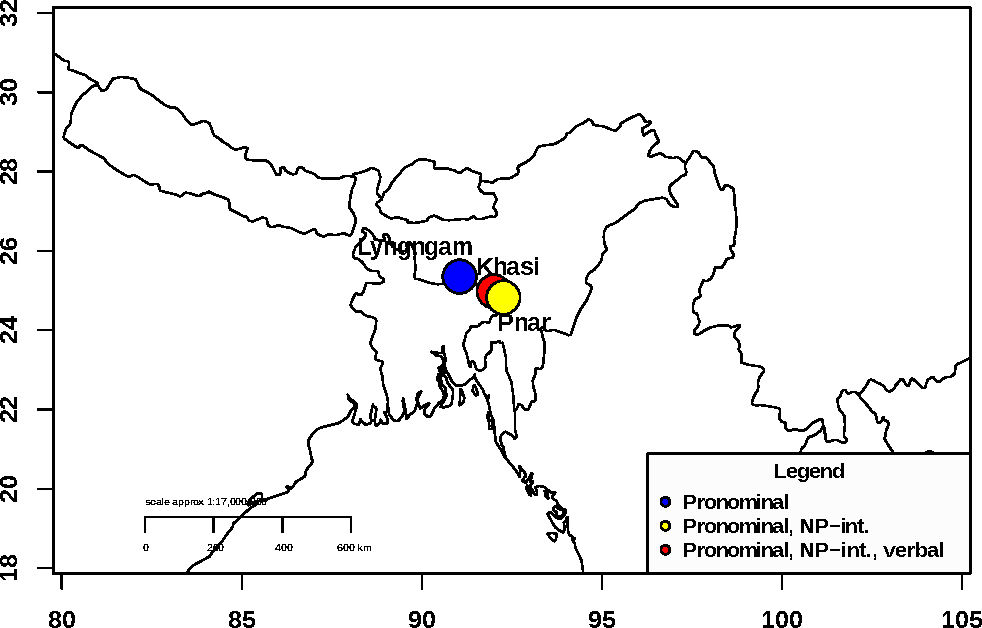
\includegraphics[width=\textwidth]{figures/11/Khasian2a.pdf}
\caption{Expansion of gender agreement within Khasian}
\label{fig:dgm:Khasian1}
\end{figure}

%\ili{Michif} (scenario 2) represents a rather unique instance of the effects of language contact dynamics on the diachrony of gender systems, and on language structures in general.

\ili{Michif} (scenario 2) is a nearly extinct mixed language originated through intense contact and multilingual practices between female \ili{Cree}  speakers and male \ili{French} speaking fur trade workers (thoroughly described by \citealt{Bakker1997}). As a result of these intriguing dynamics of language contact and transmission, the lexicon and morphosyntax of \ili{Michif} are split into two: nominal lexicon and morphosyntax are \ili{French}-based while verbal lexicon and morphosyntax are \ili{Cree}-based. Accordingly, \ili{Michif} has two co-existing gender systems, with two different systems of gender assignment \textendash{} sex-based and animacy-based \textendash{} that manifest themselves through a sharp division between gender agreement within the noun phrase and gender agreement on verbs (with the exception of demonstratives, which comply to the verb-phrase agreement pattern). The noun-phrase gender system is taken from \ili{French}, while the verb-phrase gender system is based on \ili{Cree}. This unique split system of gender agreement is illustrated in (\ref{ex:dgm:10:Michif}) where the controller noun for `mare' triggers feminine agreement within the noun phrase and animate agreement on the verb.

\ea\label{ex:dgm:10:Michif}
\langinfo {Michif} {Mixed Language, Canada and US} {\citealt[87]{Bakker1997}}\\
\gll la \v{z}yma: ki:-aja:w-e:w \~{\ae} p\v{c}i pul\~{\ae} \\
\textsc{def.an.f.sg} mare \textsc{pst-}have-\textsc{ta.3$ \rightarrow $3\textsuperscript{i}} \textsc{indef.an.m.sg} little foal \\
\glt `The mare had a foal.'
%\gll desde antitites na tiempo esta gof bunit-u na siuda i ya Hag\r{a}t\^na. \\
%since \textsc{red:}before \textsc{link} time already very nice-\textsc{nf} \textsc{link} town \textsc{def} \textsc{TN} Hag\r{a}t\^na \\
%\glt `A very long time ago,  Hag\r{a}t\^na was a very pretty town already'.
%\z
\z

%The emergence of this \textit{unique} type of expanded gender agreement system can be understood only within the \textit{unique} contact dynamics that characterize the origin of \ili{Michif} as a mixed language.

The last instance of expanding gender agreement systems in our sample is Makanza \ili{Lingala} (scenario 3). In this variety of \ili{Lingala}, non-sex-based, arbitrary gender distinctions (and corresponding gender agreement patterns) were reintroduced during the standardization process that the language underwent between 1901 and 1902 under the influence of the Scheutist missionaries, who wanted to create an official language that looked more like a `proper \ili{Bantu} language'. \ili{Kinshasa Lingala}, which is nowadays the most widely spoken variety of \ili{Lingala} and which did not undergo the standardization process attested in Makanza \ili{Lingala}, exhibits a heavily reduced gender system where gender distinctions and gender agreement patterns are exclusively animacy-based. This reduced gender system is the result of the pidginization and creolization processes that are at the very origins of the history of \ili{Lingala}, which is the historical descendent of the \ili{Bangala} pidgin, developed at the \ili{Bangala} state post on the northwestern banks of the Congo River (for more details on the history of different varieties of \ili{Lingala} and their gender systems see \citealt{Bokamba1977,DiGarbo2016,Meeuwis2013}).

To summarize, our data suggest that the patterns of change through which languages may acquire more domains of gender inflection tend to be rather heterogeneous and language-specific. However, the limited number of cases examined here does not allow us to formulate any far reaching generalization on the dynamics of gender agreement expansion. While this calls for further investigation, patterns of gender agreement expansion will not be discussed further in the remainder of the paper.

\section{How simple/complex are gender agreement systems on the rise and/or in decline?}
\label{sec:dgm:simple/compl}
In \sectref{sec:dgm:evolution}, we brought up two hypotheses about the complexity of gender systems.  Firstly, in viewing the complexity of gender as an evolving variable, instances of gender systems in decline could be considered as reducing complexity and instances of gender systems on the rise/under expansion as emerging/increasing complexity. Secondly, both reducing and rising gender systems could be expected to show less complexity than their full-fledged counterparts. The data presented in this paper do not, however, support these hypotheses. In this section, we show that many of the processes of reduction and emergence of gender agreement attested in our data contribute to increase the complexity of gender systems as matched against the proposed measures of gender complexity.


Starting with reducing gender agreement, we suggest that especially in those cases in which patterns of reduction only affect sub-parts of the agreement system, whether as a result of morphophonological erosion or of redistribution of agreement, this cannot be described as a straightforward simplification process. In Standard \ili{Swedish}, for instance, the merger between the Masculine and Feminine genders in the domain of noun-phrase internal agreement gave rise to: (1) a sex-based, referential system of gender assignment, which is active only in the domain of pronominal agreement and for nouns that denote entities at the top end of the animacy hierarchy (humans and, occasionally, higher animals); (2) a non-sex-based, semantic and formal type of gender assignment system, which is active through agreement in the domain of adnominal modification. When mapped onto the model of gender complexity proposed by \citet{Audring2017},  this split in the type of classificatory distinctions that agreement targets are sensitive to qualifies as an increase in gender complexity, as illustrated in (\ref{ex:dgm:10:Audring}). (The symbol ``{\textless}'' here, as well as in (\ref{ex:dgm:11:Audring2}), (\ref{ex:dgm:12:Audring3}) and (\ref{ex:dgm:13:Audring4}), reads as ``less complex than''.)

\eabox[-.5\baselineskip]{\label{ex:dgm:10:Audring}
\fittable{
\parbox[t]{13cm}{Split agreement system and gender complexity (\citealt[adapted from][]{Audring2017})}\\
}

\vspace{3mm}
\fittable{
\parbox[t]{13cm}{Matching values (between targets) {\textless} Mismatching values (between targets)}}}

This effect can be analyzed as a violation of the Principle of Independence in that the type and number of gender distinctions available in a language vary depending on the type of agreement targets that inflect for gender.  Mismatching gender values across different types of targets need to be separately specified in the description of a gender system, which leads to an increase in description length and thus in complexity.

Similarly, we saw that the redistribution of agreement is usually triggered by the reanalysis of the gender assignment of hybrid nouns. In the Asia Minor \ili{Greek} dialects, for instance, the critical items are nouns that are grammatically masculine or feminine, but semantically denote inanimate entities. In some Asia Minor \ili{Greek} varieties (such as Pontic),\il{Greek, Pontic} the ongoing reanalysis of the gender assignment rules associated with these nouns is reflected through mismatching agreement patterns whereby targets adjacent to nouns retain syntactic agreement and non-adjacent targets agree semantically. In Audring's model of gender complexity, hybrid nouns qualify as a ``complexifying phenomenon in a gender system'' because they engender mismatches in the agreement patterns that they control. This is schematized in (\ref{ex:dgm:11:Audring2}) and (\ref{ex:dgm:12:Audring3}).

\ea\label{ex:dgm:11:Audring2}
Hybrid nouns and gender complexity (\citealt{Audring2017})\\

\vspace{3mm}
Consistent controller {\textless} Hybrid controller
\z

\ea\label{ex:dgm:12:Audring3}
Semantic agreement and gender complexity (\citealt{Audring2017})\\

\vspace{3mm}
Targets do not have a choice in value {\textless} Targets have a choice in value
\z

When, due to mismatches between grammatical gender and semantic properties of hybrid nouns, agreement targets have a choice in value, these choices need to be specified in the description of a gender system. This increases the description length of the system, and thus its complexity.

Conversely, when the reduction, loss or semantic reanalysis of gender agreement patterns are more pervasive, this usually results in an uncontroversial simplification of the gender agreement system. Under morphophonological erosion, this is for instance the case of \ili{English}, where sex-based gender distinctions are only preserved on third personal and possessive pronouns and index purely semantic distinctions.\footnote{On the use of the pronouns `he' and `she' with inanimate referents in varieties of American and Australian \ili{English} see \citet{Pawley2004}.}  Under agreement redistribution, this is the case of Rumeic\il{Greek, Rumeic} Greek, where the gender system has become completely semanticized. Nouns denoting male entities are masculine, nouns denoting female entities are feminine, and nouns denoting inanimate entities are neuter.

Moving on to the emergence of gender agreement, the young gender systems examined in this paper also exhibit some features of high complexity when measured against the dimensions proposed by \citet{Audring2017}.  We observe that, under contact-induced gender emergence, only a subset of lexical items within a given word class (nouns and/or adjectives) is sensitive to
gender distinctions. For instance, in \ili{Chamorro}, only property words borrowed from \ili{Spanish} can inflect for gender, and there is a great deal of intraspeaker variation as for how productively gender agreement is used. Similarly, in \ili{Nalca}, where the emergent gender system is the result of a language internal development, gender marking is also not fully productive, and it can be switched off whenever certain syntactic conditions within the noun phrase are not met.  Low productivity and optionality in gender marking count as complexifying factors according to \citet{Audring2017}: they introduce variability in the gender agreement system of a language as a result of lexical and/or grammatical idiosyncrasies that are, in fact, independent of gender.


\ea\label{ex:dgm:13:Audring4}
Low productivity and gender complexity (\citealt{Audring2017})\\

\vspace{3mm}
Gender marking is obligatory {\textless} Gender marking is optional

\vspace{3mm}
Gender marking is fully productive  {\textless} Only a subset of lexical items per agreement target mark gender

\z

When gender is not fully obligatory or fully productive, specifying explicitly under which circumstances gender marking occurs adds to the system's description length, which means higher complexity. Conversely, the emergent gender systems examined in this paper are rather simple with respect to domains of gender agreement, given that they all display one agreement target, which in all cases examined is confined to the domain of adnominal modification.

Reducing and emerging gender systems represent transitional stages between the \textit{absence of gender} and \textit{full-fledged gender systems}, two rather stable stages in the history of individual languages and language families. These transitional stages are to a large extent associated with phenomena that, we think, increase gender complexity as a side-effect of ongoing language change. In the case of gender reduction, we observed, for instance, a pervasive occurrence of mismatching agreements, which is due to the fact that innovations (a) do not immediately reach all available agreement targets, but rather spread gradually across agreement domains; and (b) do not immediately affect all controller nouns, but rather those with ambiguous semantics (that is, hybrid nouns) first. Under gender emergence, gender agreement tends to be non-obligatory and thus non-frequent. Therefore the main factors underlying increased complexity in reducing and emerging gender systems are partial distributions and optionality, which are ultimately connected to ongoing variation and change.\footnote{This has also been pointed out to us by Jenny Audring.} While we hope to have shown that some crosslinguistically recurrent patterns can be associated with these systems in transition, we think that their relative stability is harder to generalize over and depends on the interplay between internal and external dynamics of change, the understanding of which falls outside the scope of this paper.


%\label{sec:dgm:demography}
\section{Concluding remarks and prospects for future research}
\label{sec:dgm:conclusion}
We consider the main contribution of this paper to be bringing diachrony in focus in the typological study of gender complexity.
We hope to have shown that investigating closely related languages enables us to formulate empirically grounded diachronic inferences about the decline, rise and expansion of gender agreement, as well as about how these dynamics of change affect the complexity of gender systems. In particular, we found that both gender agreement patterns in decline and gender agreement patterns on the rise feature properties of increased complexity when assessed against existing gender complexity metrics. We suggested that emerging and declining patterns of gender agreement represent transitional stages between two poles: genderless languages and full-fledged gender agreement systems. These poles often appear as less complex than the transitional stages, as represented in our sample. Whether this can be generalized over all cases of emerging and declining gender systems is a hypothesis that should be tested on a larger data set and, possibly, with the support of quantitative methodologies.

We think that one additional contribution of this paper is to have shown that implicational hierarchies can be used as schemas for investigating complexity variation across languages in a meaningful way, not only at the synchronic level (as previously suggested by \citealt{Miestamo2009}), but also diachronically. In this respect, we found that, in the languages of our sample, the agreement domains at the two opposite ends of the Agreement Hierarchy, attributive modifiers and personal pronouns, often function as the place from which processes leading to both the rise and the decline of gender agreement begin. Furthermore, our data suggest that at least the reduction and loss of gender agreement tend to be directional in nature, and that the type of directionality at stake is predicted by whether loss and reduction are due to morphophonological erosion or redistribution of agreement patterns.

We hope that these results may spark further research on the relationship between the complexity of gender systems and other well-known implicational universals in the domain of gender marking, such as the series of implicational universals on the availability of gender distinctions in the plural as opposed to the singular (e.g., Universal 37), or in pronouns as opposed to nouns (e.g., Universal 43), formulated by \citet{Greenberg1963}. We believe that this line of research is particularly promising to shed new light on synchronic and diachronic interactions between gender and other grammatical domains, and their effect on the complexity of gender systems.





Finally, one important question that is left out from this paper is whether there are any external factors that contribute to explain why and under which conditions gender agreement systems complexify or simplify. Even though many of the instances of change discussed in this paper clearly involved language contact as a causal factor, the question of the relationship between the evolution of gender agreement systems and language ecology  was not addressed systematically here. Thus the answer to this question must be left to further studies. Our impression so far is that gender agreement patterns \textendash{} whose evolutionary dynamics we have tried to unravel in this paper \textendash{} might be a better match for the study of the sociolinguistic correlates of gender complexity than, say, sheer number of genders and/or type of assignment systems. Patterns of gender agreement directly hinge on inflectional morphology, which has so far been one of the main foci of research in testing the effects of social structures and language ecologies on the rise and transmissibility of linguistic complexity.



\section*{Acknowledgments} 
We thank two anonymous reviewers, as well as Jenny Audring, Johanna Nichols, and Bernhard W\"alchli for providing constructive comments on previous versions of the paper. For financial support, Francesca Di Garbo is thankful to the Wenner-Gren Foundations.

\section*{Special abbreviations}
\noindent The following abbreviations are not found in the Leipzig Glossing Rules:
\medskip

\noindent
\begin{tabular}{llll}
  3$ \rightarrow $3	&	3rd person animate obviative	&  	  \textsc{link}	&	linker	\\
  \textsc{an}	&	animate	& 	 \textsc{hab}	&	habitual	\\
  \textsc{cv} 	&	 consonant + vowel	&	\textsc{nf}	&	non-feminine	\\
	&	 phonotactic structure 	&	\textsc{red}	&	reduplication	\\
  \textsc{dp} 	&	default phrase gender	& \textsc{ta}	&	transitive animate verb	\\
  \textsc{inan}	&	inanimate	&	\textsc{tn}	&	toponym	\\
  \textsc{indef}	&	indefinite	&&\\
\end{tabular}

\sloppy
\printbibliography[heading=subbibliography,notkeyword=this]


%\begin{appendix}

\section*{Appendix} 
\largerpage[2]
\label{appendix}
\scriptsize{The sampled genealogical units are listed by macroarea and higher levels of classification are mentioned, if applicable. (Q) indicates that, for any particular language, data have been collected through full questionnaire responses; (p.c.\@) stands for personal communication (i.e., data collected through consultation of language experts but no full questionnaire response).}
\begin{table}[h]
\scriptsize
 \begin{tabularx}{\textwidth}{l@{~}l@{~}lQ@{}} % add l for every additional column or remove as necessary
  \lsptoprule
Family by macroarea & Language &Glottocode & Source\\
\midrule
\multicolumn{4}{l}{AFRICA}\\
\midrule
\multicolumn{4}{l}{\ilit{Bantu} (\ilit{Atlantic-Congo})}\\
&\ilit{Kinshasa Lingala}& ling1263 & \citet{Bokamba1977,Meeuwis2013}\\
& Makanza \ilit{Lingala}&ling1269 & \citet{Boeck1904,Bokamba1977,Meeuwis2013}\\
\midrule
\multicolumn{4}{l}{\ilit{Ghana-Togo-Mountain} (\ilit{Atlantic-Congo})} \\
& \ilit{Selee}& sele1249 &  \citet{Agbetsoamedo2014}\\
&\ilit{Igo}&igoo1238 &  Gblem-Poidi (\citeyear{Gblem-Poidi2007}; p.c.)\\
& \ilit{Ikposo}&ikpo1238 & \citet{Soubrier2013}; Ines Fiedler (p.c.)\\
\midrule
\multicolumn{4}{l}{AUSTRALIA}\\
\midrule
\multicolumn{4}{l}{Gunwinggu (Central Gunwinyguan, \ilit{Gunwinyguan})}\\
& \ilit{Kunwinjku}&gunw1252 & \citet{Evans2003}\\
& \ilit{Kundjeyhmi}&gunw1252 & \citet{Evans2003} \\
& \ilit{Kune}&gunw1252 & \citet{Evans2003}\\
\midrule
\multicolumn{4}{l}{EURASIA}\\
\midrule
\multicolumn{4}{l}{\ilit{Khasian} (\ilit{Austroasiatic})}\\
&\ilit{Khasi}&khas1269 & Anne Daladier (p.c.)\\
&\ilit{Lyngngam}& lyng1241 & Anne Daladier (p.c.)\\
&\ilit{Pnar}&pnar1238 & Anne Daladier (p.c.)\\
\midrule
\multicolumn{4}{l}{\ilit{Basque}}\\
&Standard \ilit{Basque}&basq1248 & \citet{Hualde2003}\\
&Lekeitio Basque\il{Basque, Lekeitio}&bisc1236  & \citet{Hualde1994}\\
\midrule
\multicolumn{4}{l}{\ilit{Balto-Slavic} (\ilit{Indo-European})}\\
& \ilit{Latvian}&latv1249 & \citet{Balode2001}, Anna Kalnaca (p.c.)\\
& Tamian \ilit{Latvian}&latv1249&\citet{Balode2001,Thomason2015,Koptjevskaja-Tamm2001}\\
\midrule
\multicolumn{4}{l}{\ilit{Greek} (\ilit{Indo-European})}\\
&Modern \ilit{Greek}&mode1248 & \citet{Karatsareas2009,Karatsareas2014} \\
&Pontic\il{Greek, Pontic} Greek & pont1253 & \citet{Karatsareas2009,Karatsareas2014} (Q)\\
&Rumeic Greek\il{Greek, Rumeic} &mari1411 & \citet{Karatsareas2009,Karatsareas2014} \\
&Cappadocian Greek\il{Greek, Cappadocian}& capp1239 & \citet{Karatsareas2009,Karatsareas2014} \\
 \bottomrule
 \end{tabularx}
 \end{table}
 \clearpage 
  \begin{table} 
\scriptsize
 \begin{tabularx}{\textwidth}{lllQ}  
 Continued &&&\\
  \toprule
 Family by macroarea &Language&Glottocode & Source\\
\midrule
\multicolumn{4}{l}{EURASIA}\\
\midrule
\multicolumn{4}{l}{Insular \ilit{Celtic} (\ilit{Indo-European})}\\
& \ilit{Irish}&iris1253 & \citet{Frenda2011}\\
& \ilit{Irish} (\ilit{Ros Much})&conn1243 & \citet{Frenda2011}\\
\midrule
\multicolumn{4}{l}{North \ilit{Germanic} (\ilit{Indo-European})}\\
&\ilit{Elfdalian}& dic (ISO)& \citet{AAkerberg2012}; \"Osten Dahl (Q)\\
&Karleby Swedish\il{Swedish, Karleby} &oste1241& \citet{Hultman1894,Hulden1972}\\
&Standard \ilit{Swedish}&swed1254&\citet{Duke2010}; Mikael Parkvall (Q)\\
\midrule
\multicolumn{4}{l}{Northwestern \ilit{Iranian} (\ilit{Indo-European})}\\
& \ilit{Eshtehardi}&esht1238& \citet{Stilotoappear,Yarshater1969}\\
&\ilit{Kafteji}&kaba1276& Stilo (\citeyear{Stilotoappear}; p.c.) \\
&\ilit{Kelasi}&kaba1276& Stilo (\citeyear{Stilotoappear}; p.c.) \\
\midrule
\multicolumn{4}{l}{\ilit{Lezgic} (\ilit{Nakh-Daghestanian})}\\
&\ilit{Archi}&  arch1244 & Michael Daniel, Nina Dobrushina (Q) \\
&\ilit{Aghul}&aghu1253& Nina Dobrushina (Q)\\
& \ilit{Udi}& udii1243& \citet{Nichols2003};Wolfgang Schulze (Q)\\
\midrule
\multicolumn{4}{l}{\ilit{Thebor} (\ilit{Bodic}, \ilit{Tibeto-Burman})}\\
& \ilit{Shumcho}& shum1243& Huber (\citeyear{Huber2011}; p.c.)\\
& \ilit{Jangshung}&jang1254& Huber (\citeyear{Huber2011}; p.c.)\\
\midrule
\multicolumn{4}{l}{NORTH AMERICA}\\
\midrule
\multicolumn{4}{l}{Mixed Language}\\
& \ilit{Michif}&mich1243&\citet{Bakker1997}\\
\midrule
\multicolumn{4}{l}{PAPUNESIA}\\
\midrule
\multicolumn{4}{l}{\ilit{Chamorro} (\ilit{Austronesian})}\\
&\ilit{Chamorro}&cham1312 &\citet{Stolz2012}\\
\midrule
\multicolumn{4}{l}{\ilit{Mek} (Nuclear-Trans-New-Guinea) }\\
&\ilit{Nalca}&nalc1240 & \citet{Waelchli2018}\\
&\ilit{Eipo}&eipo1242& \citet{Waelchli2018}\\
 \lspbottomrule
 \end{tabularx}
 \end{table}



%\end{appendix}

\end{document}
